%\section{Introdução}
\section{Árvores}

\begin{frame}

\begin{center}
{\Large Capítulo 06 -- Árvores}
\end{center}

Pontos fundamentais a serem cobertos:
\begin{columns}
\begin{column}{.3\textwidth}
\centering

  \begin{enumerate}
  \item Contexto e motivação

  \item Definição

  \item Implementações

  \item Exercícios 

\end{enumerate}  

\end{column}
\begin{column}{.7\textwidth}
\centering
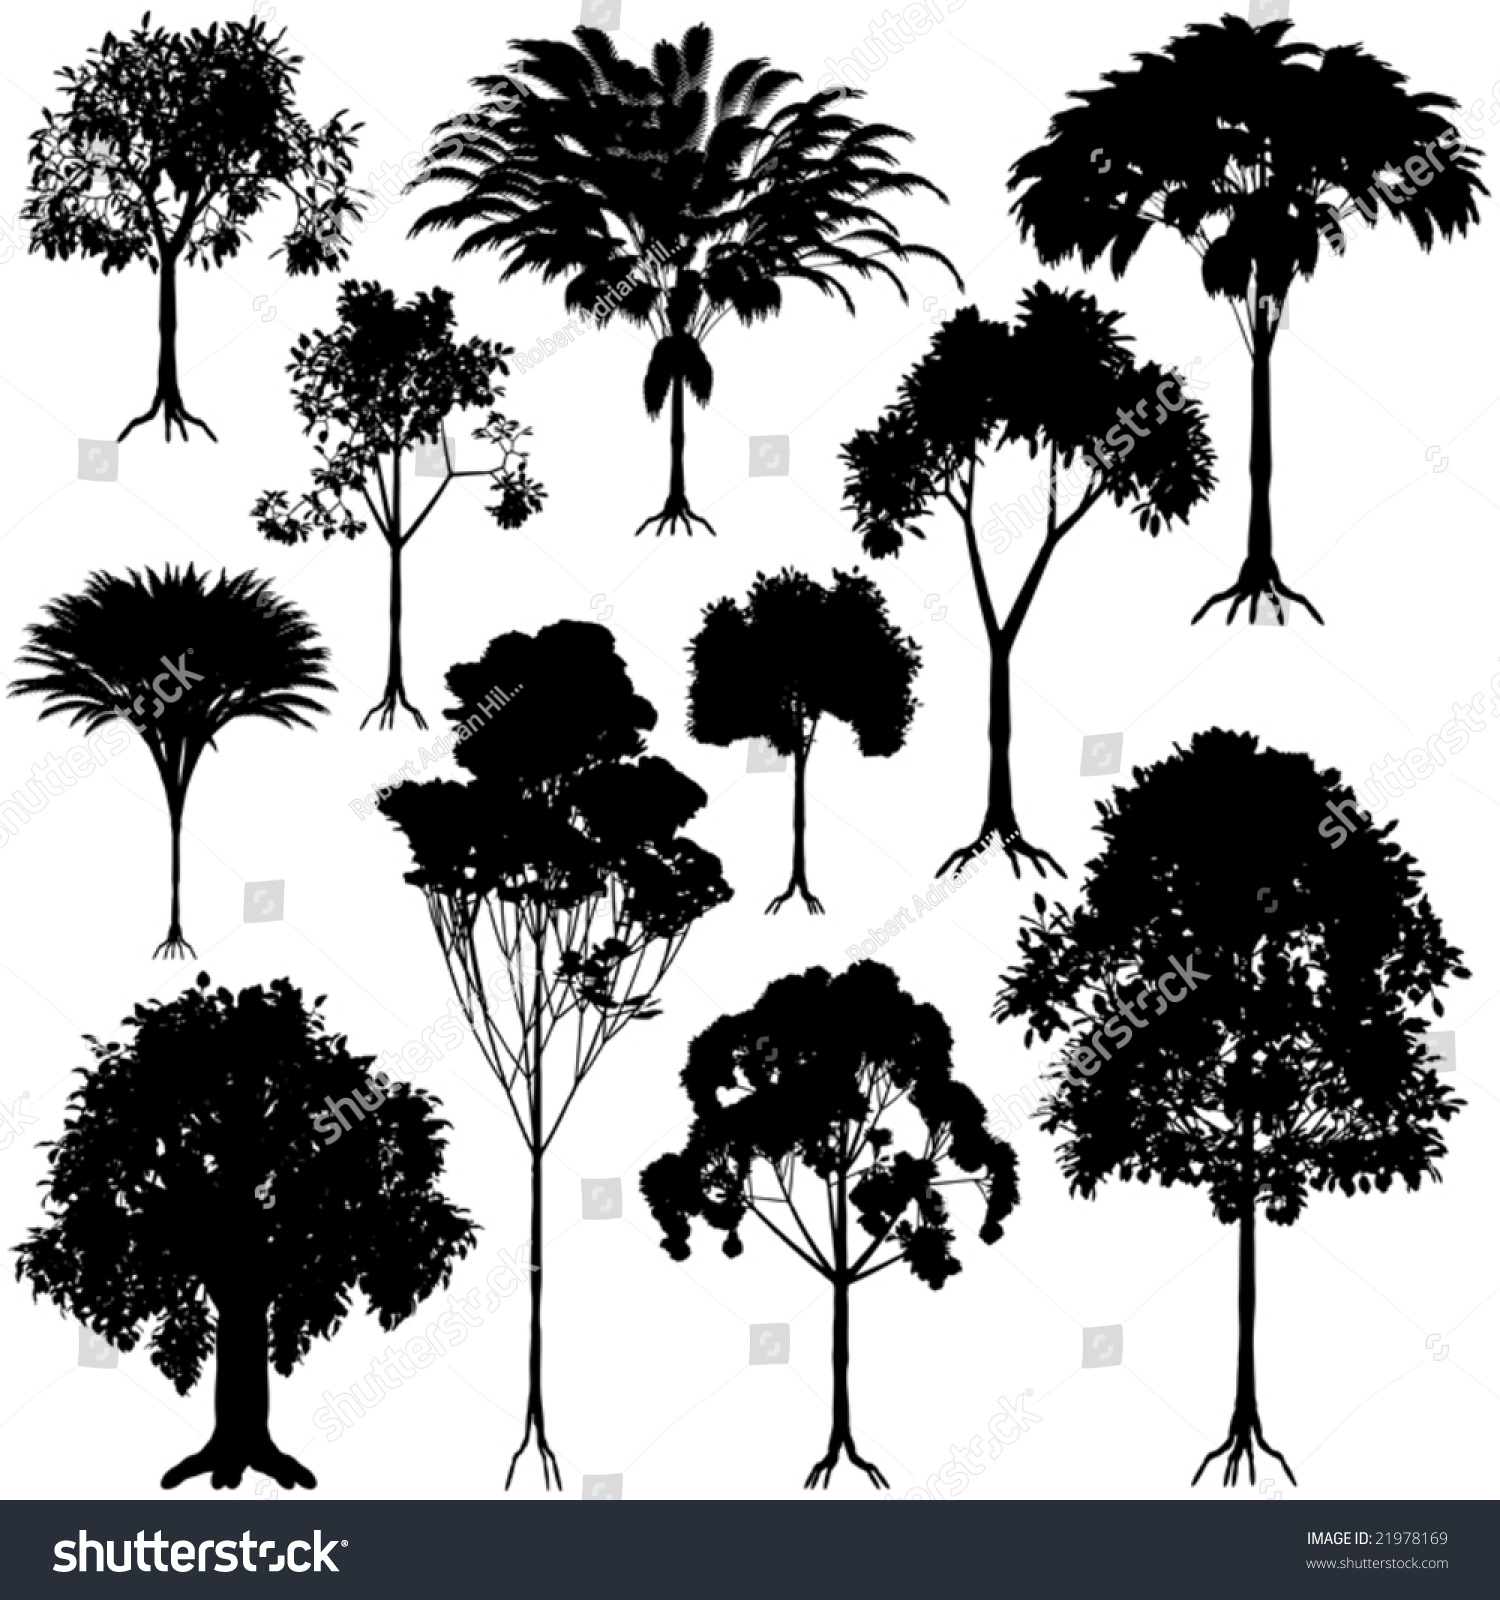
\includegraphics[height=5.3cm, width=7cm]{figs/fig_arvores/arv_CAPA.jpg}
\hspace{+0.25cm}
%\scriptsize\textcolor{red}{[Tizio, Caio et al., Nature (2006)]}
\end{column}
\end{columns}


\end{frame}
%-----------------------------------------------------------------------------
\subsection{Apresentação}

\begin{frame}%[allowframebreaks=0.9, c]

    \frametitle{Definição}
    
    \begin{itemize}
    \item Uma árvore é uma estrutura hierárquica composta por nós e ligações entre eles
    \item Pode ser vista como um grafo acíclico
    \item Cada nó possui somente um pai e zero ou mais filhos
    \item Muitas definições ...
    \end{itemize}
\end{frame}

%---------------------------------------------------------
\begin{frame}%[allowframebreaks=0.9, c]
    \frametitle{Estrutura}
    
    \begin{figure}[tbp]
    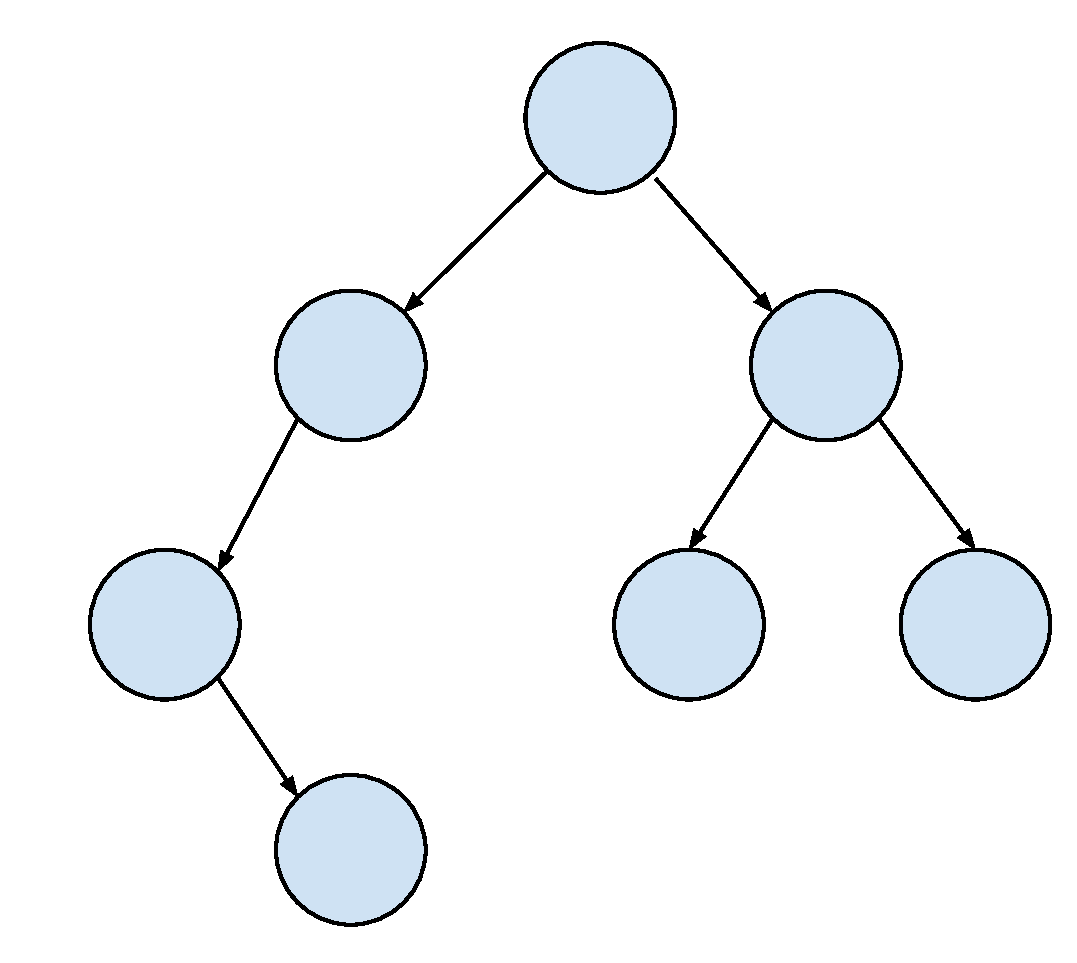
\includegraphics[keepaspectratio=true,width=2.5in]{figs/fig_arvores/arvore.pdf}
    \centering
    \caption{Exemplo de uma árvore}
    \end{figure}
\end{frame}
%---------------------------------------------------------


%---------------------------------------------------------
\begin{frame}
    \frametitle{\textit{Roadmap} para estudo}
    
\begin{block}{mantendo um \textit{foco}:}

\begin{enumerate}
  \item Conceitos de árvores genéricas etc ... 
    \item Árvores Binárias
  \item Árvore Binária de Busca
   \item Árvore AVL (iniciais dos nomes:  \textit{Georgii Adelson-Velsky et Evguenii Landis (en), 
   qui l'ont publié en 1962 sous le titre An Algorithm for the Organization of Information})
   \item Projeto 10\% : 
   \begin{itemize}
     \item  Implemente uma AVL;
    \item   Leia um conjunto de dados numéricos contidos no arquivo fornecido (um valor por linha: string, int, float, char), inserindo-os sequencialmente na AVL implementada;
    \item   Imprima o percurso (valores dos nós) em pré-ordem, em-ordem e pós-ordem, além da altura da árvore
    \item Com a altura dará para ver se a AVL está OK!
   \end{itemize}
  
  \item Vídeos bem legais no Youtube da UNIVEST
  
\end{enumerate}


\end{block}



    \end{frame}

%---------------------------------------------------------
\begin{frame}
    \frametitle{Características -- Requisitos}
    
\begin{itemize}
  
  \item  Como é um nó?
  \item  Qual o grau de um nó?
  \item  Como devem estar estruturados os valores dos nós?
  \item  O que é uma chave do nó?
  \item  O que é a altura?
  \item  Nível?
  \item  Caminhos

\end{itemize}


\end{frame}

%-------------------------------------------------------------------------------------------------------------
\begin{frame}

    \frametitle{Glossário -- 01}
    
     \begin{figure}[!ht]
     \centering
    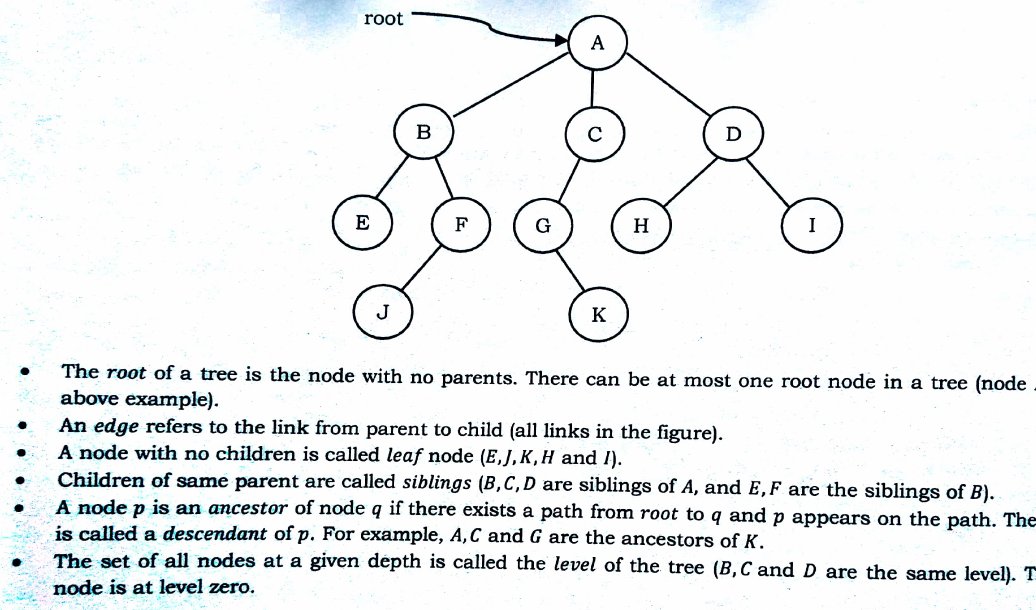
\includegraphics[width=12cm, height=7cm]{figs/fig_arvores/glossario_arv_01.png}
    %\caption{\textcolor{red}{Usando os problemas de árvores genéricas para apresentar Árvores Binárias (AB) }}
    \end{figure}

\end{frame}

%-------------------------------------------------------------------------------------------------------------
\begin{frame}

    \frametitle{Glossário -- 02}
    
     \begin{figure}[!ht]
     \centering
    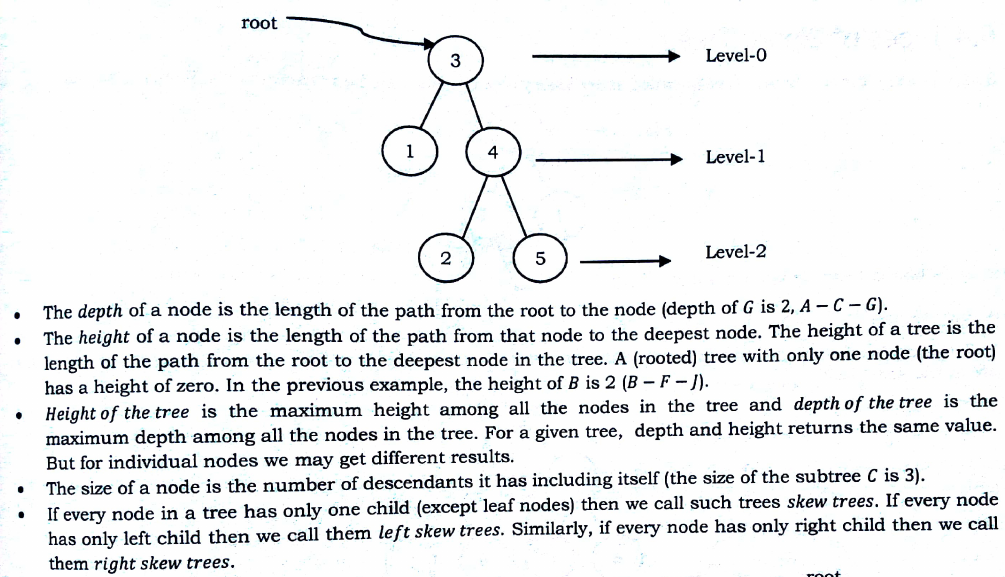
\includegraphics[width=12cm, height=7cm]{figs/fig_arvores/glossario_arv_02.png}
    %\caption{\textcolor{red}{Usando os problemas de árvores genéricas para apresentar Árvores Binárias (AB) }}
    \end{figure}

\end{frame}
%-------------------------------------------------------------------------------------------------------------
\begin{frame}

    \frametitle{Glossário -- 03}
    
     \begin{figure}[!ht]
     \centering
    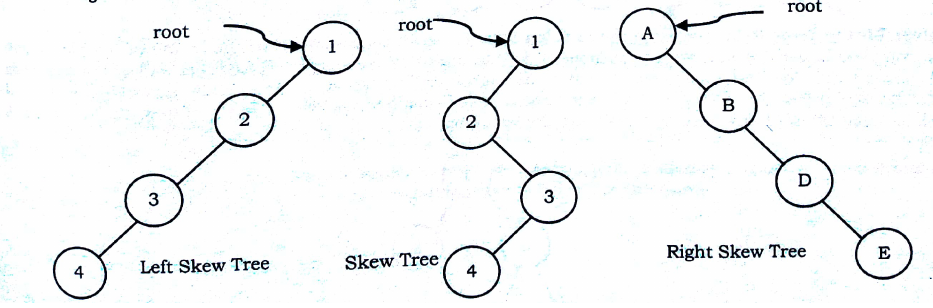
\includegraphics[width=8cm, height=5cm]{figs/fig_arvores/glossario_arv_03.png}
    %\caption{\textcolor{red}{Usando os problemas de árvores genéricas para apresentar Árvores Binárias (AB) }}
    \end{figure}

\end{frame}

%-------------------------------------------------------------------------------------------------------------

\subsection{Árvores Genéricas}

\begin{frame}

    \frametitle{Árvores Genéricas}
    %%Representação  Computacional de 
     \begin{figure}[!ht]
     \centering
    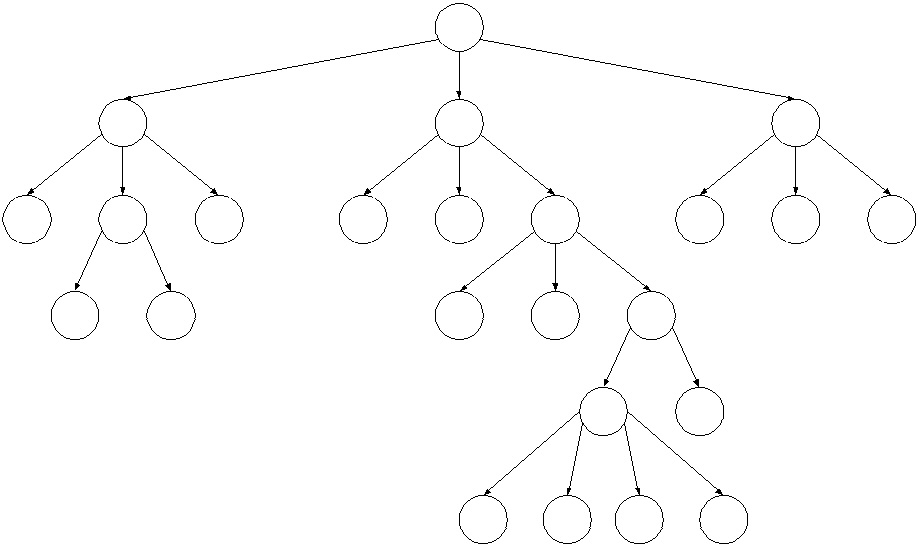
\includegraphics[width=9cm, height=5cm]{figs/fig_arvores/arv_generica01.jpg}
    \caption{\textcolor{red}{Usando os problemas de árvores genéricas para apresentar Árvores Binárias (AB) }}
    \end{figure}

\end{frame}
%-------------------------------------------------------------------------------------------------------------

\begin{frame}

    \frametitle{Transformando uma Árvore Genérica em Binária}
    
     \begin{figure}[!ht]
     \centering
    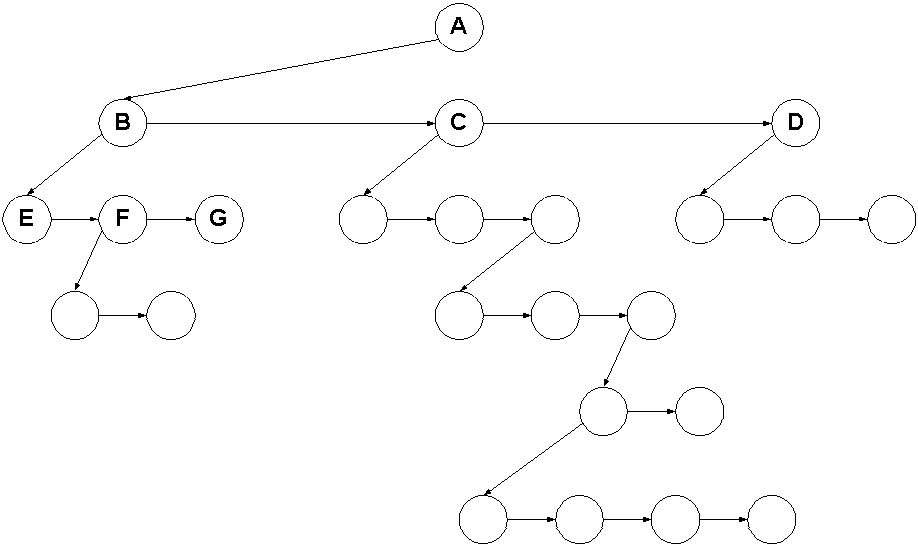
\includegraphics[width=10cm, height=5cm]{figs/fig_arvores/arv_generica02.jpg}
    \caption{\textcolor{red}{Usando os problemas de árvores genéricas para apresentar Árvores Binárias(AB)}}
    \end{figure}

\end{frame}

%-------------------------------------------------------------------------------------------------------------

\begin{frame}

    \frametitle{Representação  Computacional de uma Árvore Genérica}
    
     \begin{figure}[!ht]
     \centering
    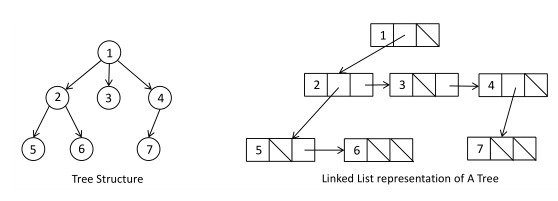
\includegraphics[width=10cm, height=5cm]{figs/fig_arvores/arv_generica03.jpg}
    \caption{\textcolor{red}{Felizmente há um algoritmo que transforme  Árvores Genéricas em Binárias (AB) }}
    \end{figure}

\end{frame}
%-------------------------------------------------------------------------------------------------------------

\begin{frame}

    \frametitle{Representação  Computacional de uma Árvore Genérica}
    
     \begin{figure}[!ht]
     \centering
    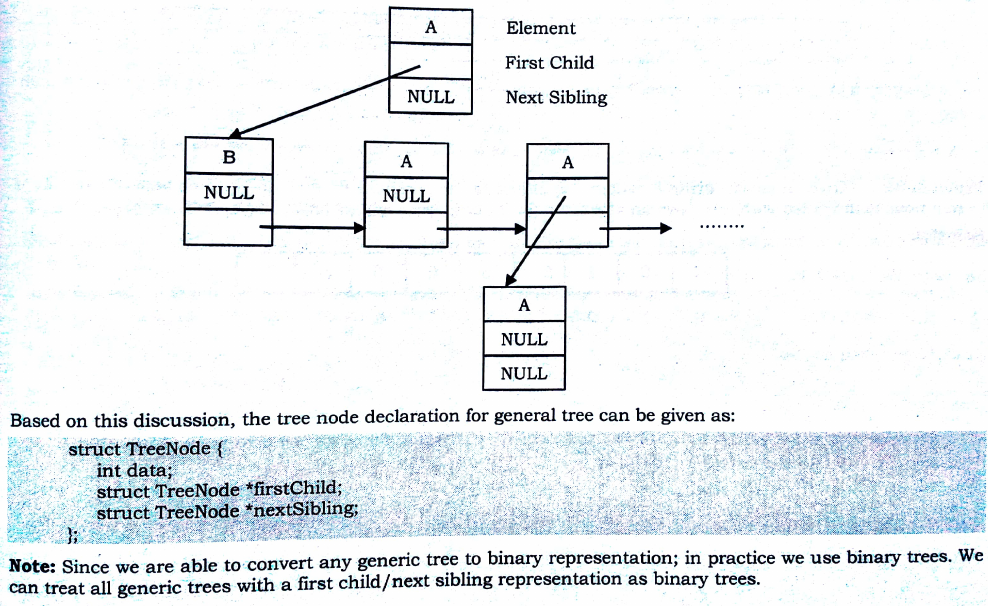
\includegraphics[width=10cm, height=6cm]{figs/fig_arvores/arv_generica04.png}
   \caption{\textcolor{red}{Veja a \textit{struct} ... lembra o quê?}}
    \end{figure}

\end{frame}

%---------------------------------------------------------

\subsection{Aplicações}

\begin{frame}

    \frametitle{Aplicações}

    \begin{itemize}
      \item  Área de compiladores: análise sintática 
      \item  Buscas com complexidade na ordem de: $O(\log n)$ 
     % \item  O uso de Árvores Genéricas foi apenas para motivar as ABBs
      \item  Na área de IA para construção de árvores de decisão: mineração de dados (\textit{big data})
      \item  Organização de taxonomias de conhecimento
      \item  Estruturas hierárquicas em geral      
      
    \end{itemize}    
    
\end{frame}


%---------------------------------------------------------

\begin{frame}

\frametitle{Aplicação  de Árvores}

  \begin{figure}[!ht]
     \centering
    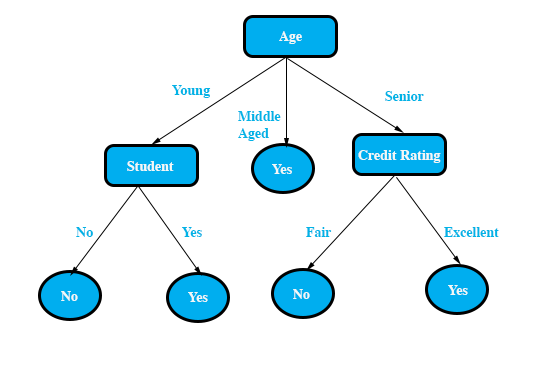
\includegraphics[width=7cm, height=5.5cm]{figs/fig_arvores/aplicacao_decision_tree.png}
    \caption{Árvore de Decisão}
    \end{figure}

\end{frame}

%---------------------------------------------------------

\begin{frame}

    \frametitle{Aplicação  de Árvores}

  \begin{figure}[!ht]
     \centering
    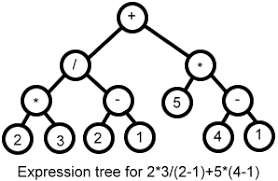
\includegraphics[width=7cm, height=5.5cm]{figs/fig_arvores/aplicacao_expression_tree.png}
    \caption{Árvores de expressões -- binárias -- novamente}
    \end{figure}

\end{frame}

%---------------------------------------------------------

\subsection{Árvore Binária de Busca}

\frame{
    \frametitle{Árvores Binárias de Buscas - ABBs}
    
    
    \begin{itemize}
      \item Árvores Genéricas (AGs): foram utilizadas para motivação as ABBs
      \item Computacionalmente, as ABBs tem um interesse maior que as AGs
      \item Assim, se inicia com ABBs, e seus algoritmos serão adaptados as AGs
    \end{itemize}
    \pause
    
\begin{block}{Definição:}
        
    Árvore onde cada nó possui até 2 filhos. O filho da esquerda só pode conter
    chaves menores do que a do pai, enquanto que o filho da direita só comporta chaves
    maiores do que a do pai.
    \end{block}

}

%---------------------------------------------------------
\frame{
    \frametitle{Árvore Binária de Busca}
    
    \begin{figure}[tbp]
    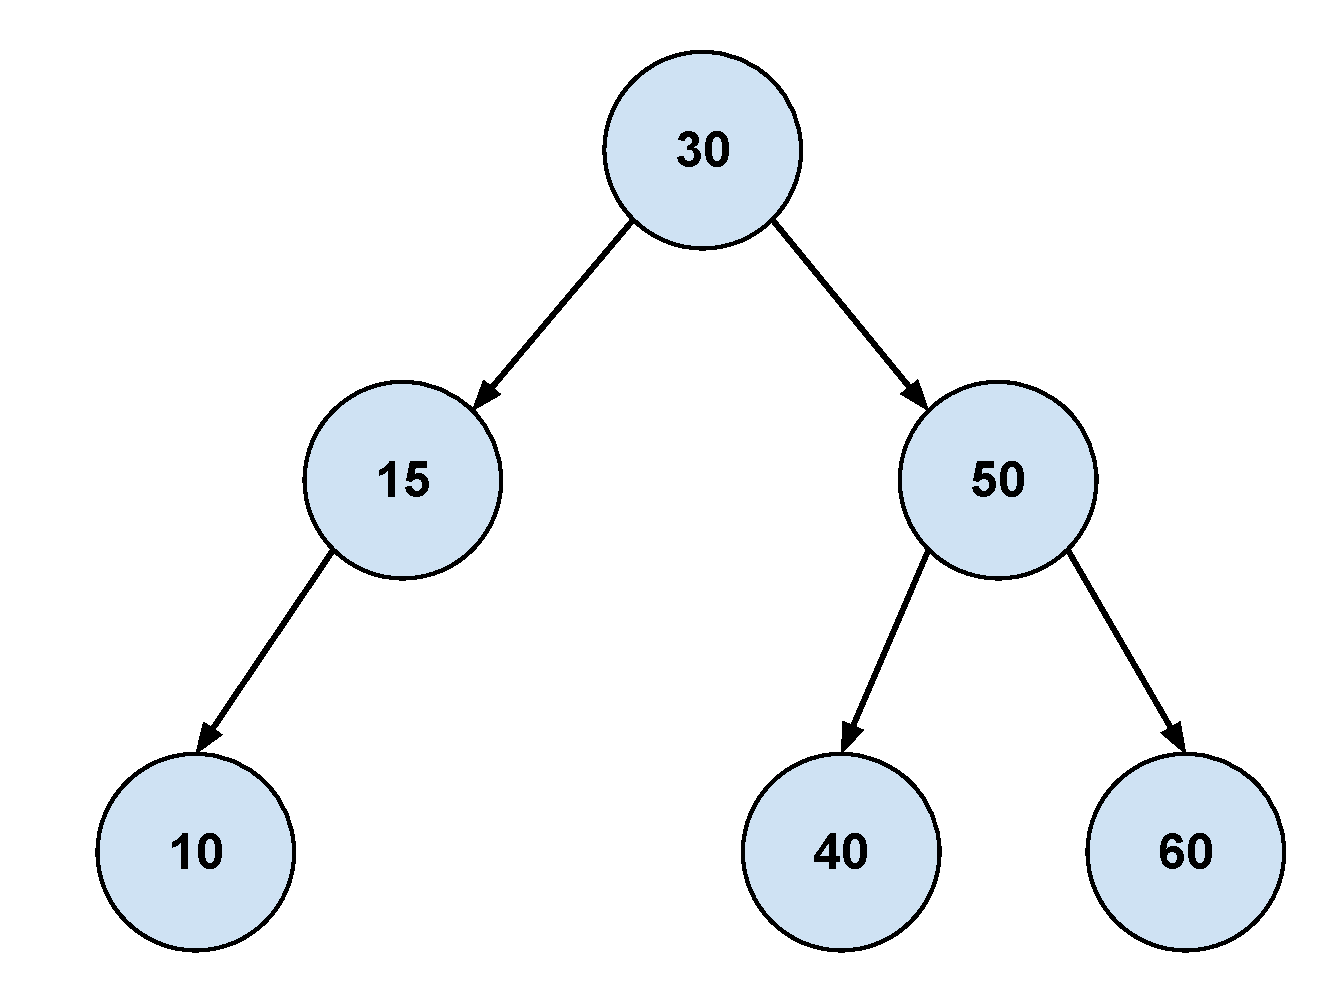
\includegraphics[keepaspectratio=true,width=3in]{figs/fig_arvores/arvore_binaria_de_busca}
    \centering
    \caption{Exemplo de árvore binária de busca}
    \end{figure}
}

%---------------------------------------------------------
\begin{frame}
    \frametitle{Árvore Binária de Busca}
    
    \begin{figure}[tbp]
    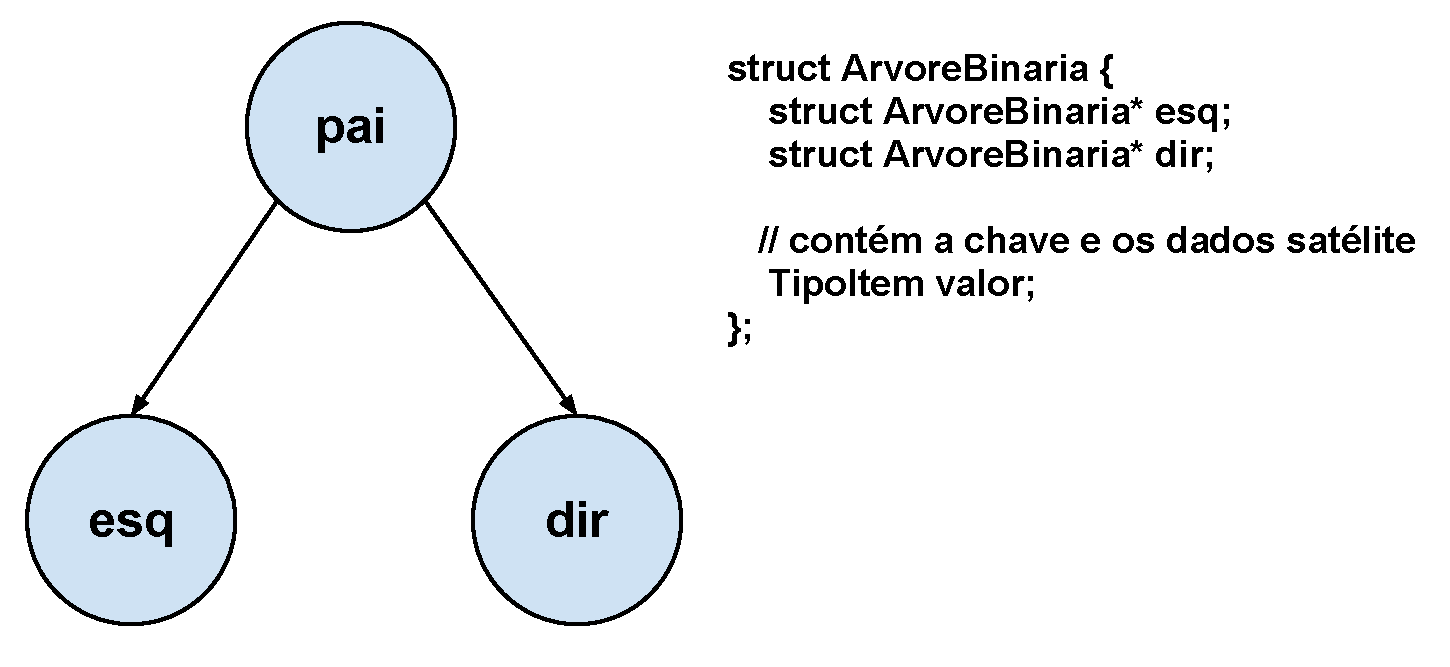
\includegraphics[keepaspectratio=true,width=4in]{figs/fig_arvores/no}
    \centering
    \caption{Estrutura básica / nó}
    \end{figure}

\end{frame}

%---------------------------------------------------------
\frame{
    \frametitle{Operações Básicas}
    
    \begin{block}{Operações Básicas}
    \begin{itemize}
    \item Inserção
    \item Busca
    \item Remoção -- faltando
    \end{itemize}
    \end{block}
    
    \begin{block}{Usos Comuns}
    \begin{itemize}
    \item Dicionários / vetores associativos
    \item Filas de prioridades
    \end{itemize}
    \end{block}
}

%---------------------------------------------------------
\frame{
    \frametitle{Complexidade Computacional}
    
    Quando a árvore está balanceada todas as três operações podem ser implementadas com complexidade
    computacional igual a $O(\log n)$.
    \\ [2em]
    No pior caso (desbalanceamento) estas operações possuem complexidade $O(n)$~\cite{cormen}.
}

%---------------------------------------------------------
\begin{frame}[fragile]
\frametitle{Árvore Binária de Busca - Inserção}
\begin{verbatim}
INSERÇÃO(ARVORE, ITEM) {
    SE ARVORE->CHAVE == NULO
       ARVORE->ITEM = ITEM
       return      //e SE CHAVE jah existente?

    SE ITEM->CHAVE < ARVORE->CHAVE
        SE ARVORE->ESQ = NULO ENTÃO
            ARVORE->ESQ = ARVORE(ITEM)
        SENÃO
            INSERÇÃO(ARVORE->ESQ, ITEM)
    SENÃO
        SE ARVORE->DIR = NULO ENTÃO
            ARVORE->DIR = ARVORE(ITEM)
        SENÃO
            INSERÇÃO(ARVORE->DIR, ITEM)
}
\end{verbatim}
\begin{itemize}
  \item 
 \textcolor{red}{Futuro: rever este pseudo-código}
  \item Vá ao fonte implementado -- insere nó

\end{itemize}

\end{frame}


\section{Percorrendo Árvores Binárias}
\begin{frame}
  \frametitle{Percorrendo Árvores Binárias}


\begin{itemize}
  \item Uma operação muito comum é percorrer uma árvore binária, o que significa passar por todos os nós, pelo menos uma vez.

 \item  O conceito de visitar significa executar uma operação com a informação armazenada no nó, por exemplo, imprimir seu conteúdo. 

 \item Na operação de percorrer a árvore pode-se passar por alguns nós mais de uma vez, sem porém visitá-los.

 \item Uma árvore é uma estrutura não seqüêncial, diferentemente de uma lista, por exemplo. Não existe ordem natural para percorrer árvores e portanto podemos escolher diferentes maneiras de percorrê-las. 

 \item  Iremos estudar três métodos para percorrer árvores. 

 \item Todos estes três métodos podem ser definidos recursivamente e se baseiam em \textbf{três operações básicas}: visitar a raiz, percorrer a subárvore da esquerda e percorrer a subárvore da direita. 

 \item A única diferença entre estes métodos é a ordem em que estas operações são executadas.
\end{itemize}

\end{frame}
%---------------------------------------------------------

\begin{frame}
  
  \frametitle{Percurso em pré-ordem}
  
O primeiro método, conhecido como percurso em pré-ordem, implica em executar recursivamente os três passos na seguinte ordem: 
 
\begin{enumerate}
  \item Visitar a raiz (imprimir esta);
 \item Percorrer a subárvore da esquerda em pré-ordem;
 \item Percorre a subárvore da direita em pré-ordem.

\end{enumerate}

\end{frame}
%---------------------------------------------------------


\begin{frame}
  \frametitle{Exemplo em pré-ordem}
  
%%% preorder transversal
%%%binary_tree_traversal.png

\end{frame}
%---------------------------------------------------------


\begin{frame}
  \frametitle{Resumo das estratégias}
  
%%% preorder transversal
%%%binary_tree_traversal.png

\end{frame}

%---------------------------------------------------------
%---------------------------------------------------------


\begin{frame}
  \frametitle{Resumo das estratégias}
  
%%% preorder transversal
%%%binary_tree_traversal.png

\end{frame}

%---------------------------------------------------------


%---------------------------------------------------------



%---------------------------------------------------------
\frame{
    \frametitle{Árvore Binária de Busca - Inserção}
    
    \begin{figure}[tbp]
    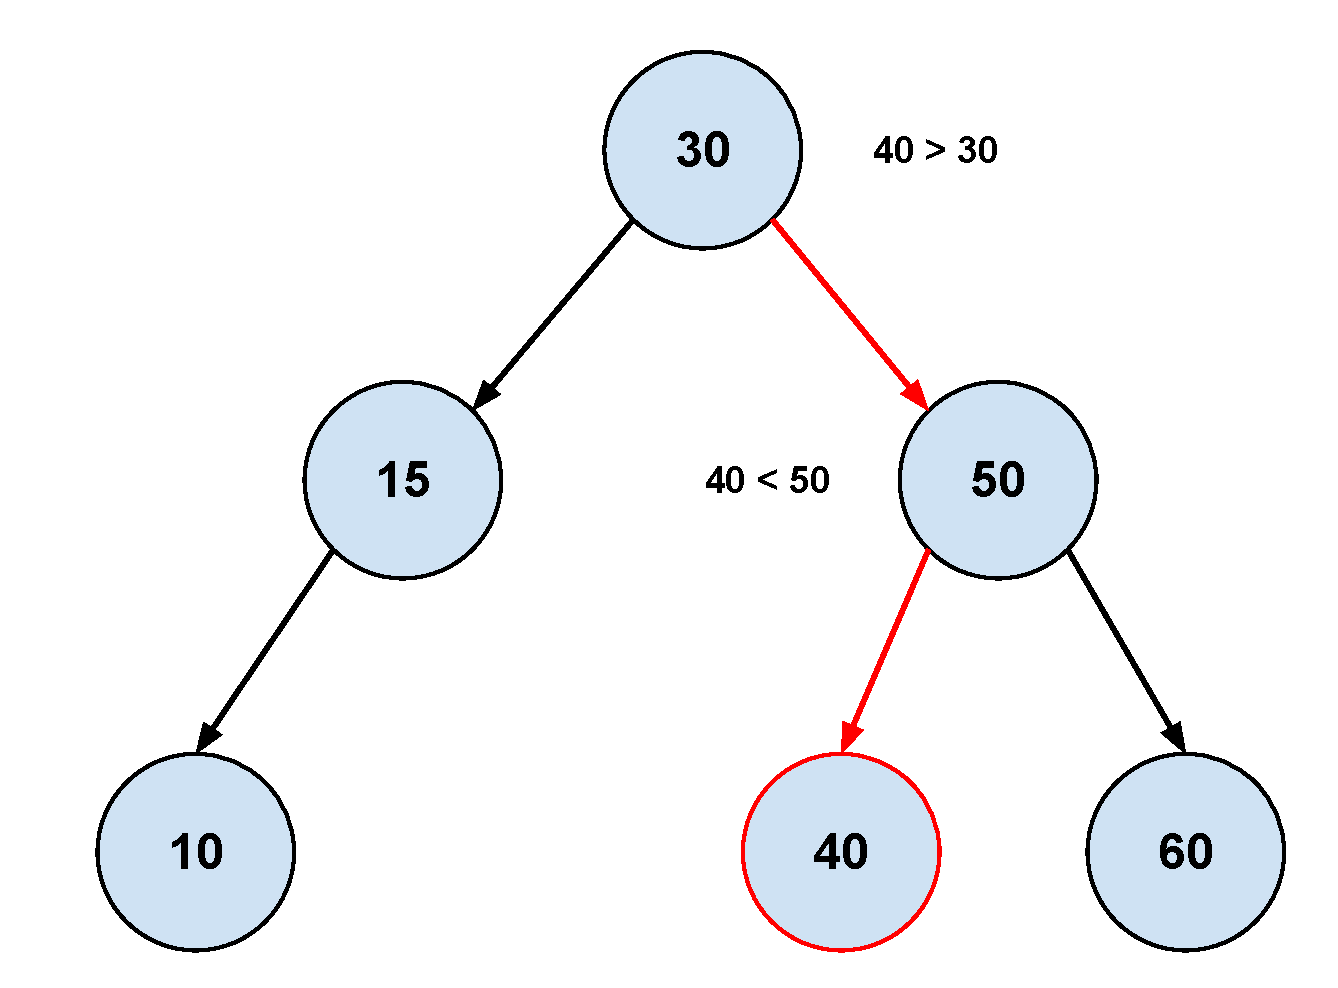
\includegraphics[keepaspectratio=true,width=3in]{figs/fig_arvores/insercao_1}
    \centering
    \caption{Exemplo de inserção da chave 40}
    \end{figure}
}

%---------------------------------------------------------
\frame{
    \frametitle{Árvore Binária de Busca - Inserção}
    
    \begin{figure}[tbp]
    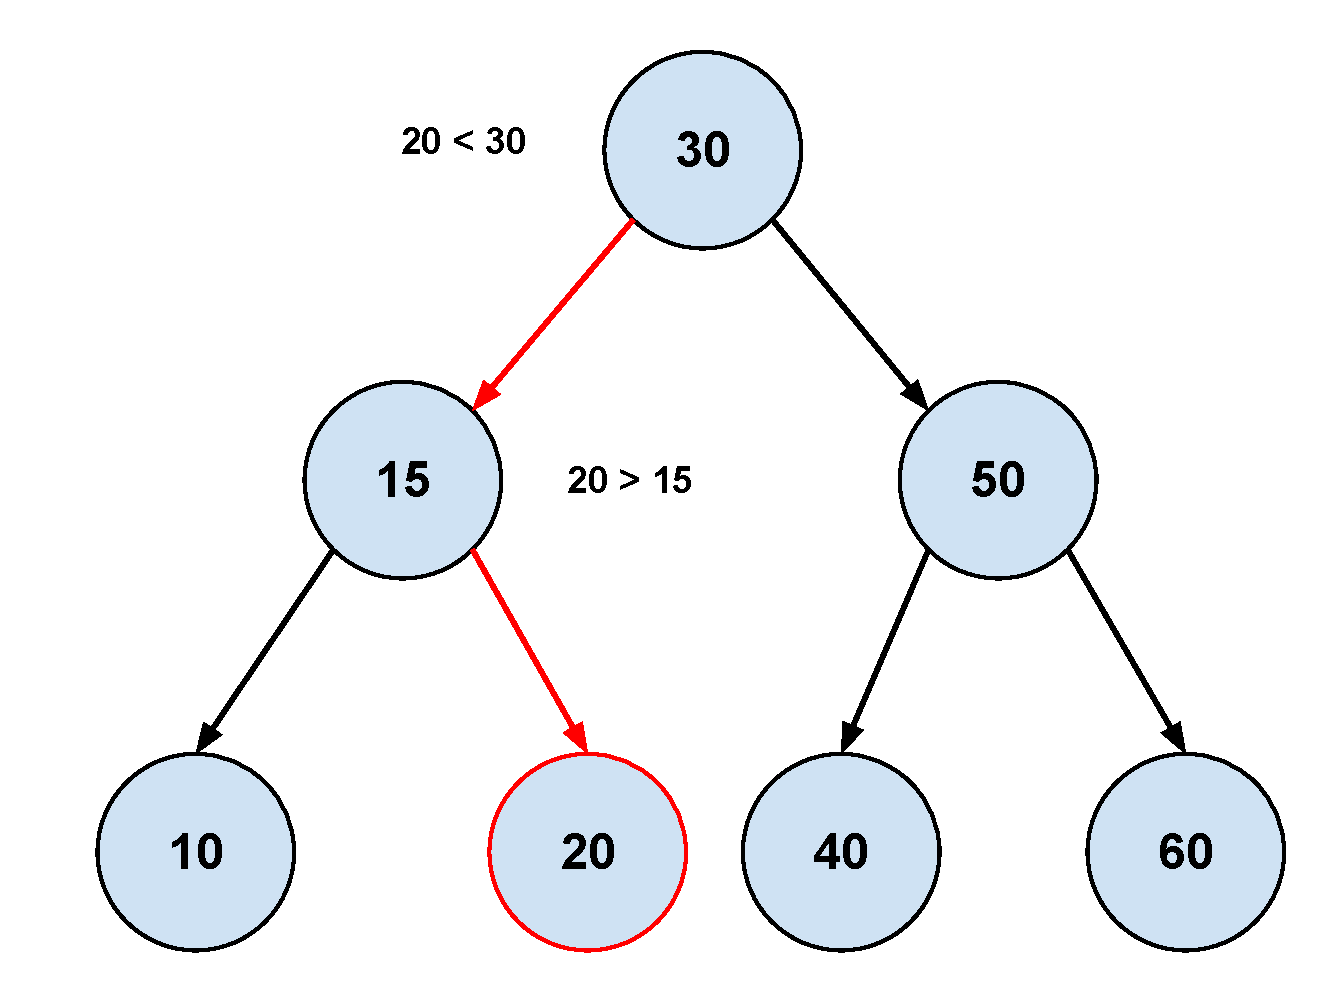
\includegraphics[keepaspectratio=true,width=3in]{figs/fig_arvores/insercao_2}
    \centering
    \caption{Exemplo de inserção da chave 20}
    \end{figure}
}

%---------------------------------------------------------
\begin{frame}[fragile]
\frametitle{Árvore Binária de Busca - Busca}
\begin{verbatim}
BUSCA(ARVORE, CHAVE) {
    SE ARVORE = NULO
        return NULO
        
    SE ARVORE->CHAVE = CHAVE
        return ARVORE
    
    SE CHAVE < ARVORE->CHAVE
        return BUSCA(ARVORE->ESQ, CHAVE)
    SENÃO
        return BUSCA(ARVORE->DIR, CHAVE)
}
\end{verbatim}
\end{frame}

%---------------------------------------------------------
\frame{
    \frametitle{Árvore Binária de Busca -- Remoção}
    
    A remoção de um nó se enquadra em um dos seguintes casos:
    
    \begin{enumerate}
    \item Remoção de um nó folha (nenhum filho)
    \item Remoção de um nó com somente um filho
    \item Remoção de um nó com dois filhos
    \item  \textcolor{red}{Faltam as figuras ainda .... vários slides}
    \end{enumerate}

   %% O tratamento de cada caso foi apresentado em sala de aula.
}

%---------------------------------------------------------
\subsection{Balanceamento}

\frame{
    \frametitle{Balanceamento}
    
    Uma árvore binária de busca balanceada garante operações de busca, inserção e
    remoção com complexidade O($\log n$), onde $n$ é o número de nós, o que a torna atrativa
    para diversas aplicações.
    \\[1em]
    Determinadas sequências de inserções ou remoções podem fazer com que uma ABB fique
    desbalanceada, tornando suas operações O($n$).
}

\begin{frame}[fragile]
\frametitle{Cálculo da Altura}
\begin{verbatim}
ALTURA(ARVORE) {
    SE ARVORE = NULO
        return -1
        
    A1 = ALTURA(ARVORE->DIR)
    A2 = ALTURA(ARVORE->ESQ)
    
    return maior(A1, A2) + 1
}
\end{verbatim}

\end{frame}

%---------------------------------------------------------
\begin{frame}
\frametitle{Cálculo da Altura}

\begin{figure}[tbp]
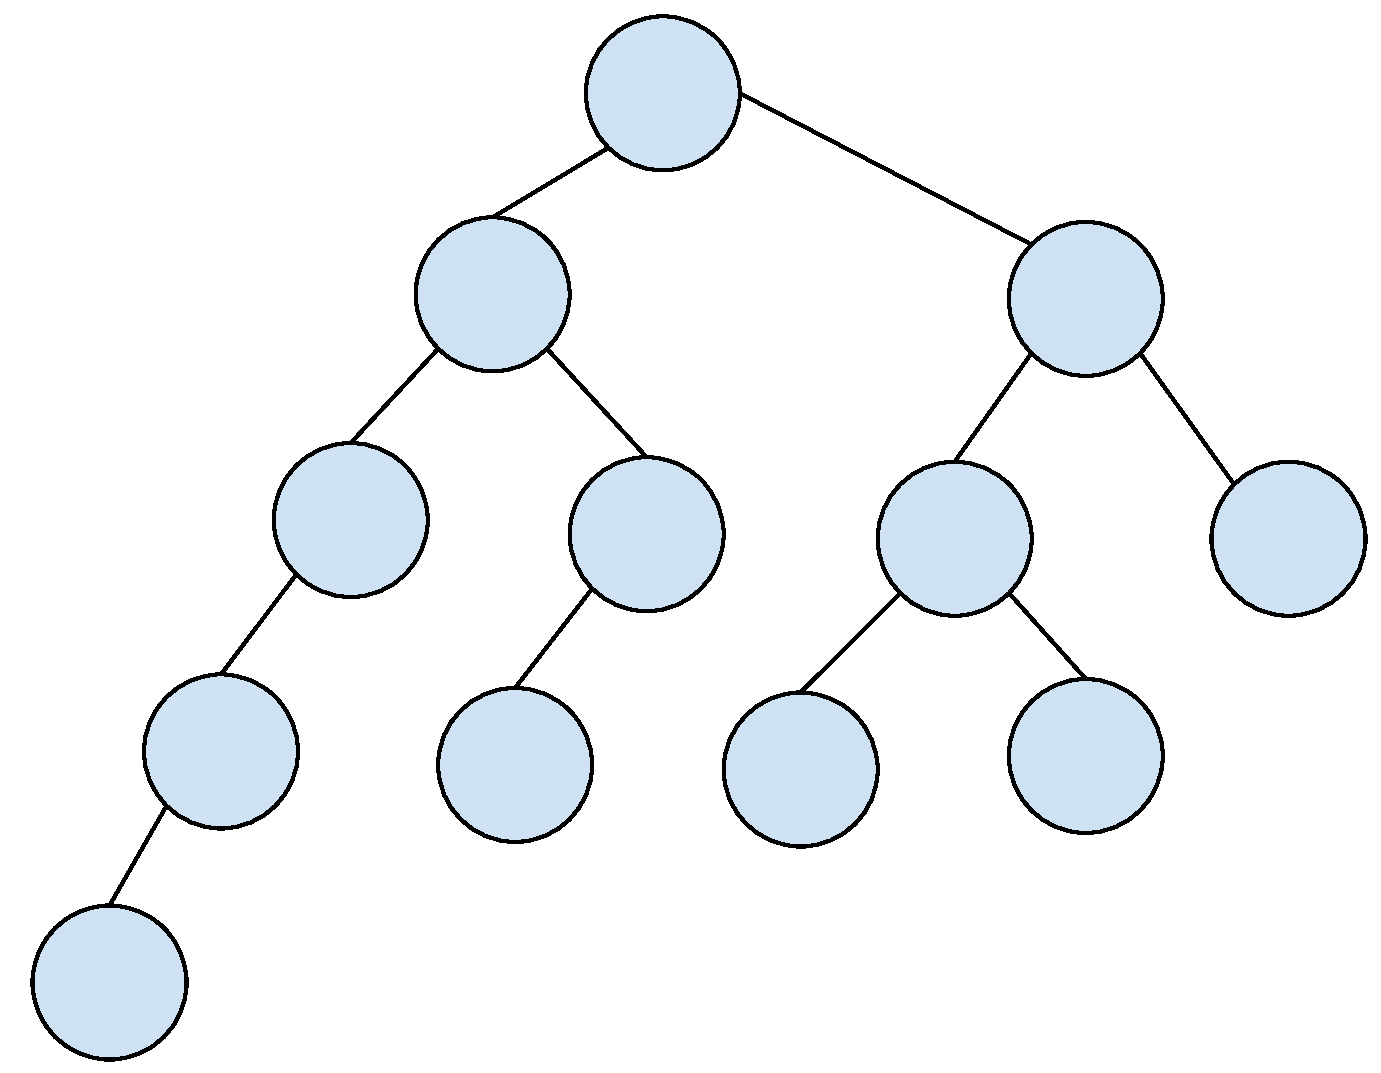
\includegraphics[keepaspectratio=true,width=3in]{figs/fig_arvores/altura1}
\centering
\caption{Exercício: determine a altura de cada subárvore.}
\end{figure}

\end{frame}

%---------------------------------------------------------
\begin{frame}
\frametitle{Cálculo da Altura}

\begin{figure}[tbp]
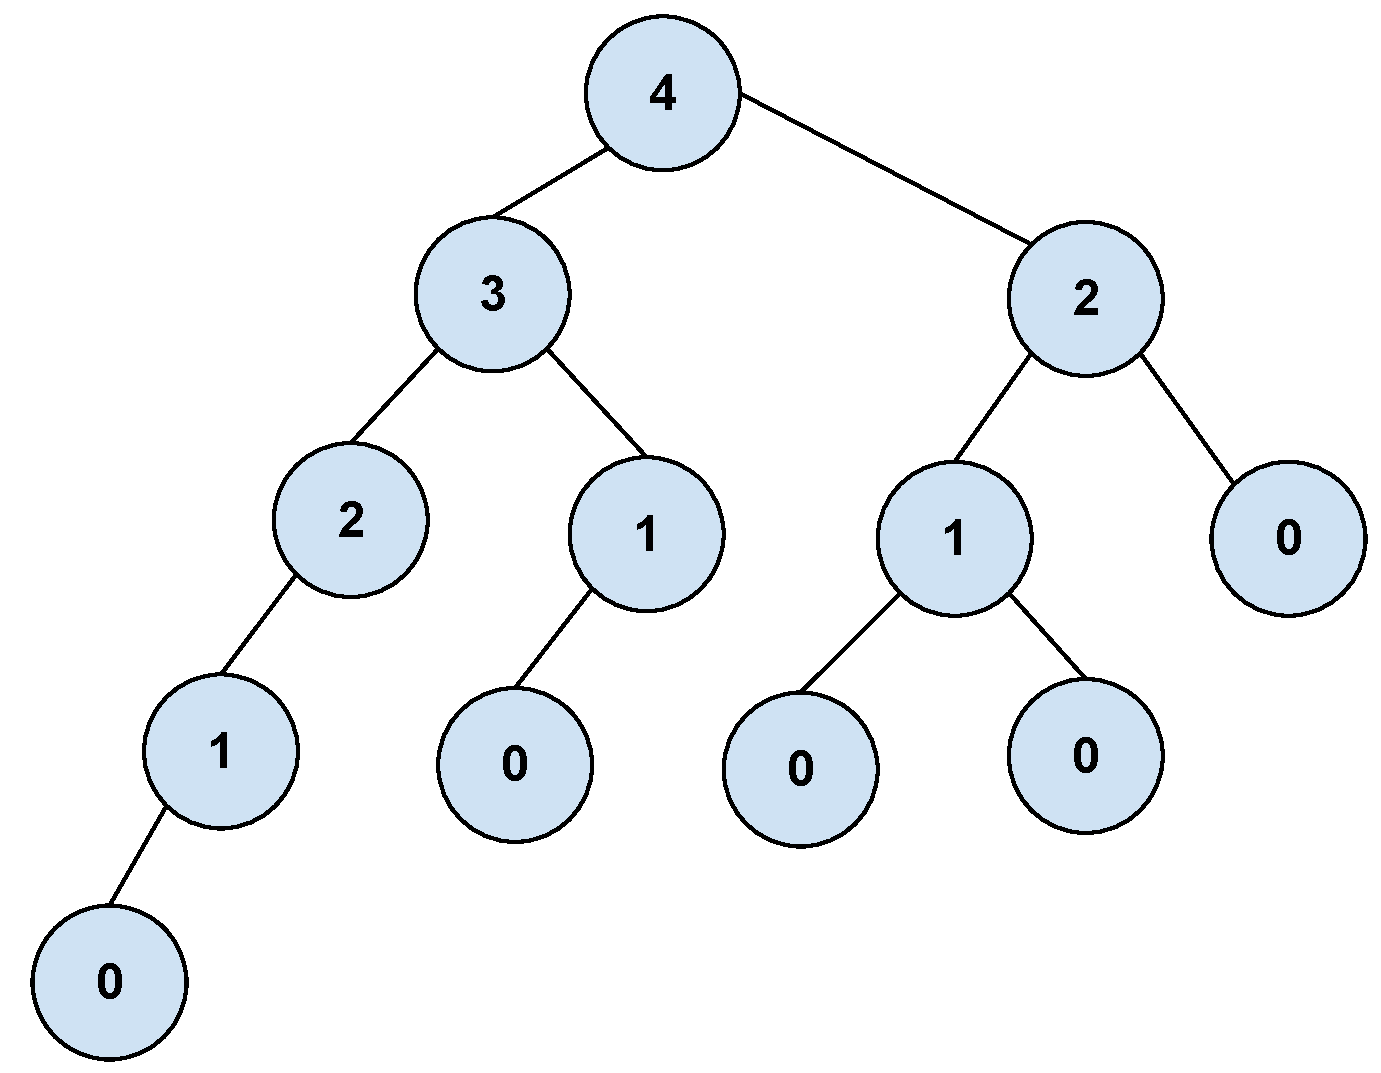
\includegraphics[keepaspectratio=true,width=3in]{figs/fig_arvores/altura2}
\centering
\caption{Resposta do exercício.}
\end{figure}

\end{frame}

%---------------------------------------------------------
\begin{frame}[fragile]
\frametitle{Cálculo do Fator de Balanceamento}
\begin{verbatim}
FB(ARVORE) {
    A1 = ALTURA(ARVORE->ESQ)
    A2 = ALTURA(ARVORE->DIR)
    return A1 - A2 
}
\end{verbatim}
\end{frame}

%---------------------------------------------------------
\frame{
    \frametitle{Balanceamento}
    
    \begin{itemize}
    \item Uma ABB está balanceada quando cada nó possui um FB igual a -1, 0 ou 1
    \item Uma inserção ou remoção pode tornar uma árvore desbalanceada, necessitando de rotações
    para o seu balanceamento
    \end{itemize}
}

%---------------------------------------------------------
\begin{frame}
    \frametitle{Exemplo de ABB Balanceada}
    
    \begin{figure}[tbp]
    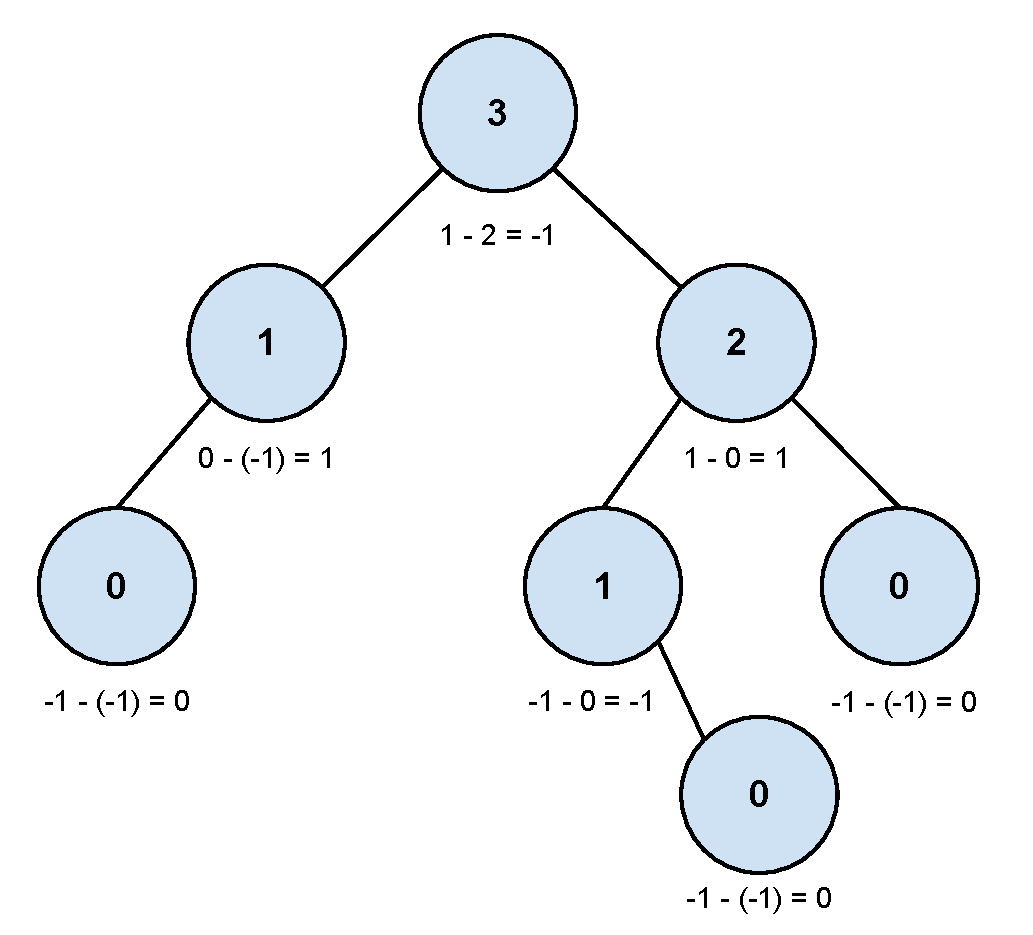
\includegraphics[keepaspectratio=true,width=3in]{figs/fig_arvores/Balanceamento_Arvore}
    \centering
    \end{figure}
\end{frame}

%---------------------------------------------------------
\begin{frame}
    \frametitle{Exemplo de ABB Desbalanceada}
    
    \begin{figure}[tbp]
    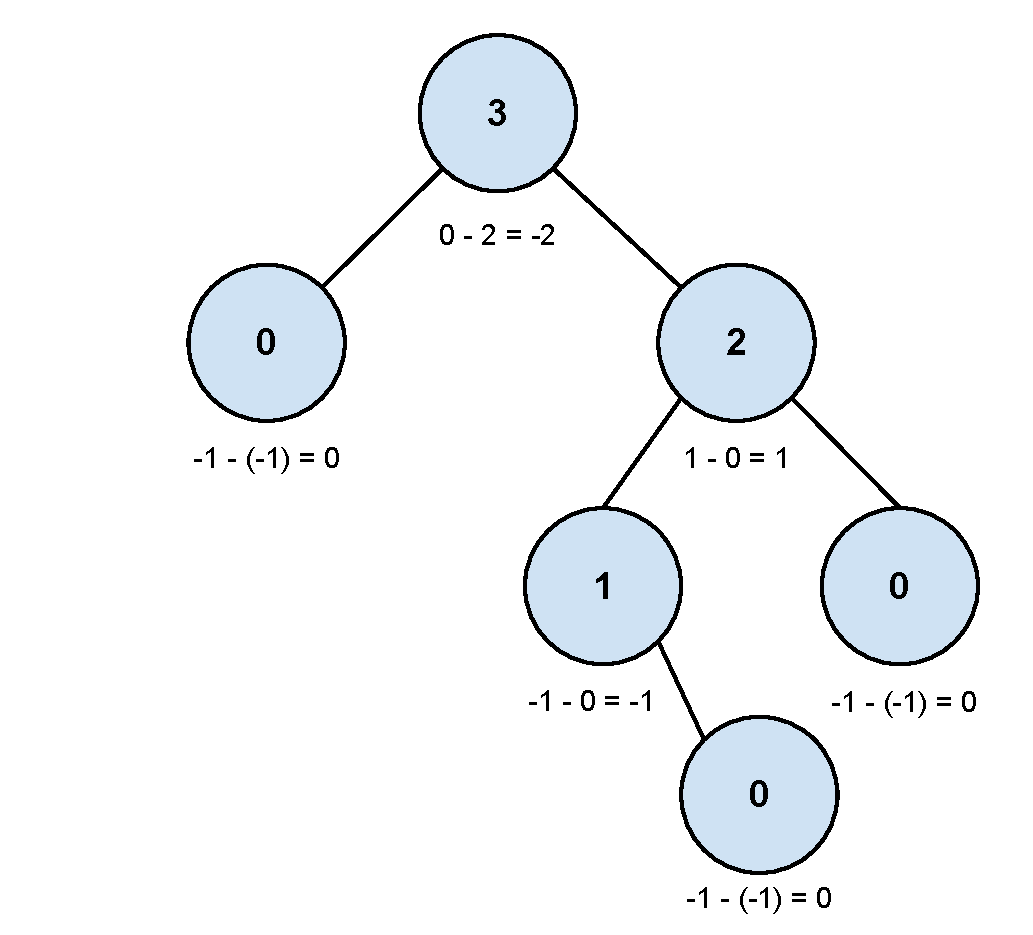
\includegraphics[keepaspectratio=true,width=3in]{figs/fig_arvores/Arvore_Desbalanceada}
    \centering
    \end{figure}
\end{frame}

%---------------------------------------------------------
\subsection{Rotações}

\begin{frame}[fragile]
\frametitle{Operação de rotação}

\begin{verbatim}
ROTACAO_DIREITA(RAIZ) {
    PIVO      = RAIZ->ESQ
    RAIZ->ESQ = PIVO->DIR
    PIVO->DIR = RAIZ
    RAIZ      = PIVO
}
\end{verbatim}

\begin{verbatim}
ROTACAO_ESQUERDA(RAIZ) {
    PIVO      = RAIZ->DIR
    RAIZ->DIR = PIVO->ESQ
    PIVO->ESQ = RAIZ
    RAIZ      = PIVO
}
\end{verbatim}
\end{frame}

%---------------------------------------------------------
\begin{frame}
    \frametitle{Rotação para Direita}
    
    \begin{figure}[tbp]
    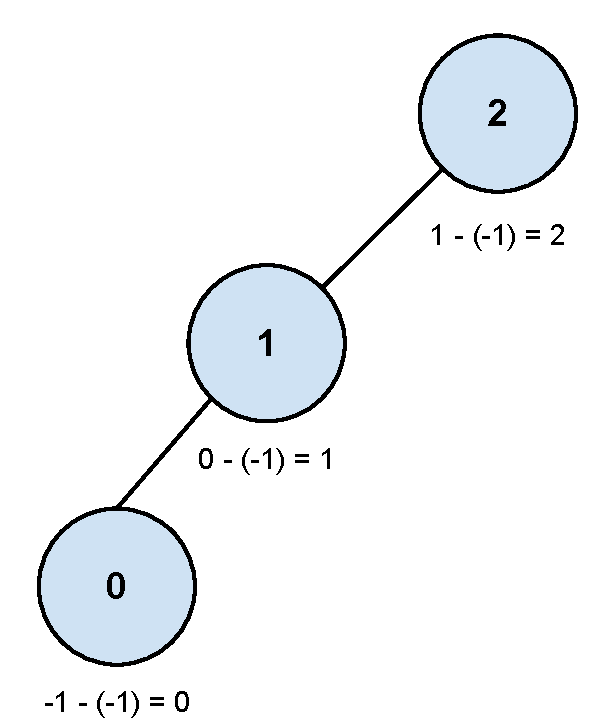
\includegraphics[keepaspectratio=true,width=2.2in]{figs/fig_arvores/Balanceamento_Arvore2}
    \centering
    \end{figure}
\end{frame}

%---------------------------------------------------------
\begin{frame}
    \frametitle{Rotação para Direita}
    
    \begin{figure}[tbp]
    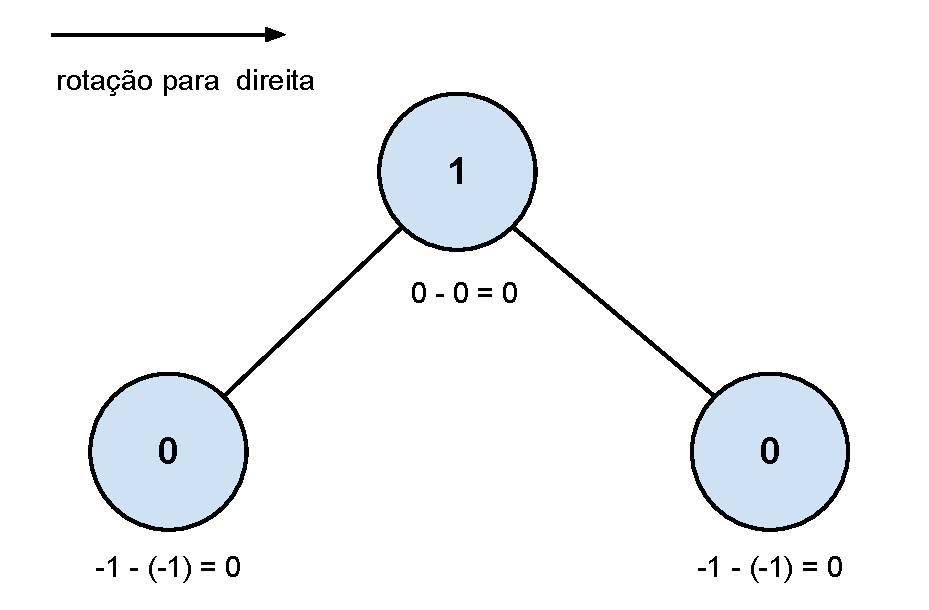
\includegraphics[keepaspectratio=true,width=3.5in]{figs/fig_arvores/Balanceamento_Arvore3}
    \centering
    \end{figure}
\end{frame}


%---------------------------------------------------------
\begin{frame}
    \frametitle{Rotação para Esquerda}
    
    \begin{figure}[tbp]
    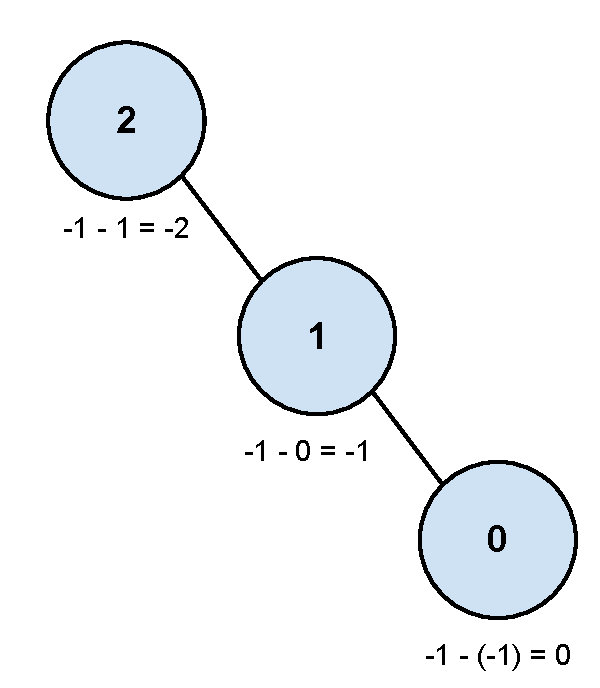
\includegraphics[keepaspectratio=true,width=2.2in]{figs/fig_arvores/Balanceamento_Arvore4}
    \centering
    \end{figure}
\end{frame}

%---------------------------------------------------------
\begin{frame}
    \frametitle{Rotação para Esquerda}
    
    \begin{figure}[tbp]
    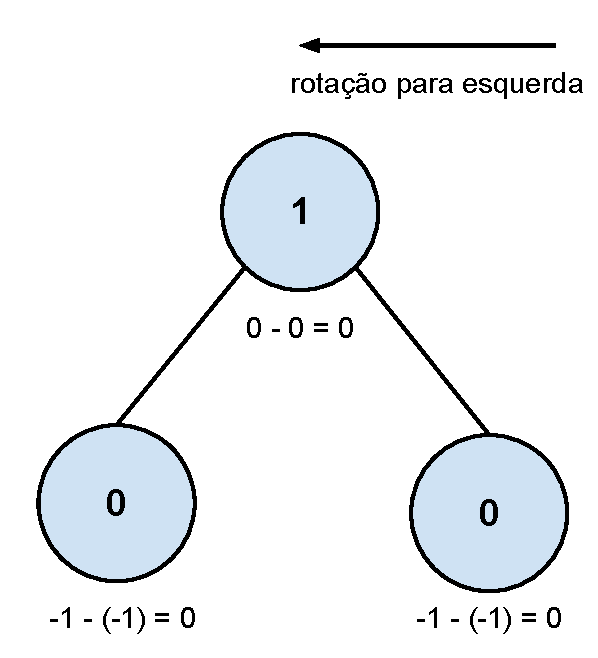
\includegraphics[keepaspectratio=true,width=2.2in]{figs/fig_arvores/Balanceamento_Arvore5}
    \centering
    \end{figure}
\end{frame}

%---------------------------------------------------------
\subsection{Árvores AVL}

\begin{frame}
    \frametitle{Árvores AVL}
    
    \begin{itemize}
    \item \textbf{AVL} desenvolvida por G. M. \textbf{A}delson-\textbf{V}elskii and E. M. \textbf{L}andis
    \item Garante o balanceamento da árvore ao realizar rotações após cada inserção ou remoção na ABB
    \end{itemize}
\end{frame}

%---------------------------------------------------------
\begin{frame}[fragile]
\frametitle{Balanceamento - Inserção}
\begin{verbatim}
BALANCEAMENTO(RAIZ) {
    SE FB(RAIZ) = -2 ENTÃO
        SE FB(RAIZ->DIR) = -1 ENTÃO
            ROTACAO_ESQUERDA(RAIZ)
        SENÃO
            ROTACAO_DIREITA(RAIZ->DIR)
            ROTACAO_ESQUERDA(RAIZ)
    SENÃO SE FB(RAIZ) = 2 ENTÃO
        SE FB(RAIZ->ESQ) = 1 ENTÃO
            ROTACAO_DIREITA(RAIZ)
        SENÃO
            ROTACAO_ESQUERDA(RAIZ->DIR)
            ROTACAO_DIREITA(RAIZ)
}
\end{verbatim}
\end{frame}

%---------------------------------------------------------
\begin{frame}[fragile]
\frametitle{Balanceamento - Inserção}

\begin{itemize}
\item Para que a árvore tenha um bom desempenho, é essencial que o balanceamento seja
calculado eficientemente, isto é, sem a necessidade de percorrer toda a árvore após cada
modificação
\item Manter a árvore estritamente balanceada após cada modificação tem seu preço (desempenho).
Árvores AVL são utilizadas normalmente onde o número de consultas é muito maior do que o número de inserções
e remoções e quando a localidade de informação não é importante
\end{itemize}
\end{frame}

%---------------------------------------------------------
\subsection{Árvore de Espalhamento}

\frame{
    \frametitle{Árvore de Espalhamento}
    
    \begin{itemize}
    \item Reestrutura a árvore em cada operação de inserção, busca ou remoção por meio de operações de rotação
    \item Nome original: \emph{splay tree}~\cite{tarjan}. Não confundir com a Árvore N-Ária de Espalhamento (ANE) criada por professores da UDESC
    \end{itemize}
}

%---------------------------------------------------------
\frame{
    \frametitle{Árvore de Espalhamento}
    
    \begin{itemize}
    \item Evita a repetição de casos ruins [O(n)] devido ao seu rebalanceamento natural
    \item Não realiza o cálculo de fatores de balanceamento, simplificando sua implementação
    \item Pior caso para uma operação se mantém O(n), mas, ao considerar uma cadeia de operações,
    \emph{garante} uma complexidade amortizada de O($\log$n) para suas operações básicas
    \end{itemize}
}

%---------------------------------------------------------
\frame{
    \frametitle{Árvore de Espalhamento}
    
    \begin{itemize}
    \item Se baseia na operação de espalhamento, que utiliza rotações para mover uma determinada
    chave até a raiz
    \item A sua complexidade O($\log$ n) em uma análise amortizada é garantida pelas rotações efetuadas, o que
    a difere do uso simples de heurísticas como o \emph{mover para a raíz}
    \end{itemize}
}

%---------------------------------------------------------
\frame{
    \frametitle{Exemplo - Espalhamento pela chave 1}
    
    \begin{figure}[tbp]
    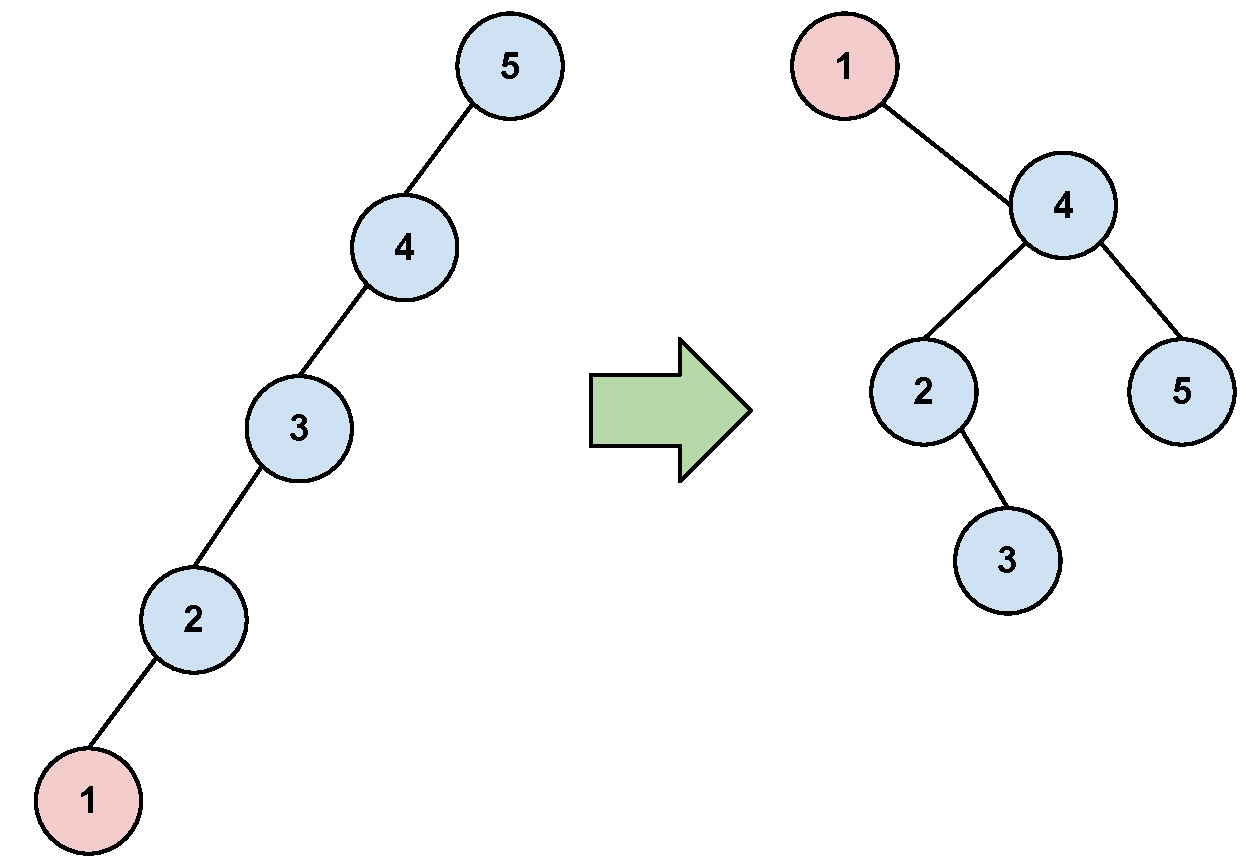
\includegraphics[keepaspectratio=true,width=3.5in]{figs/fig_arvores/Espalhamento}
    \centering
    \end{figure}
}

%---------------------------------------------------------
\frame{
    \frametitle{Operações Básicas}
    
    \begin{description}
    \item[Espalhamento] Move a chave desejada para a raiz por uma
    sequência bem definida de operações de rotação
    \item[Busca] Busca uma chave na árvore
    \item[Inserção] Insere uma nova chave na árvore
    \item[Remoção] Remove uma chave da árvore
    \end{description}
}

%---------------------------------------------------------
\frame{
    \frametitle{Operações Básicas}
    
    \begin{itemize}
    \item Uma árvore de espalhamento é uma árvore binária de busca válida,  logo operações como os percursos (pré, em e pós ordem) são idênticas as operações
    em uma ABB
    \item As operações de inserção, busca e remoção podem ser definidas com base
    na operação de espalhamento
    \end{itemize}
}

%---------------------------------------------------------
\begin{frame}[fragile]
\frametitle{Árvore de Espalhamento - Busca}
\begin{verbatim}
BUSCA(RAIZ, CHAVE) {
    return ESPALHAMENTO(RAIZ, CHAVE)
}
\end{verbatim}
\end{frame}

%---------------------------------------------------------
\begin{frame}[fragile]
\frametitle{Árvore de Espalhamento - Inserção}
\begin{verbatim}
INSERE(RAIZ, CHAVE) {
    INSERE_ABB(RAIZ, CHAVE)
    return ESPALHAMENTO(RAIZ, CHAVE)
}
\end{verbatim}
\end{frame}

%---------------------------------------------------------
\begin{frame}[fragile]
\frametitle{Árvore de Espalhamento - Remoção}
\begin{verbatim}
REMOVE(RAIZ, CHAVE) {
    RAIZ = ESPALHAMENTO(RAIZ, CHAVE)
    
    SE RAIZ->DIR ENTÃO
        AUX = ESPALHAMENTO(RAIZ->DIR, CHAVE)
        AUX->ESQ = RAIZ->ESQ
    SENÃO
        AUX = RAIZ->ESQ
    
    return AUX
}
\end{verbatim}
\end{frame}

%---------------------------------------------------------
\frame{
    \frametitle{Estratégias de Espalhamento}
    
    Duas estratégias:
    
    \begin{description}
    \item[Bottom-Up] Parte do nó acessado e o movimenta para a raiz da árvore por meio de rotações
    \item[Top-Down] Parte do nó raiz, rotacionando e \emph{removendo do caminho} os nós entre a raiz e o nó desejado, armazenando-os
    em duas árvores auxiliares, remontando a árvore completa na sua etapa final.
    \end{description}
}

%---------------------------------------------------------
\frame{
    \frametitle{Espalhamento Bottom-Up}
    
    \begin{itemize}
    \item Na estratégia Bottom-Up, a operação de espalhamento realiza
    rotações subindo gradativamente de níveis, a partir da chave desejada
    \item Enquanto a chave não estiver na raiz, deve-se verificar qual o
    caso aplicável (ZIG, ZIG-ZIG ou ZIG-ZAG) e realizar as rotações necessárias
    \end{itemize}
}

%---------------------------------------------------------
\frame{
    \frametitle{Caso 1: ZIG}
    
    \begin{figure}[tbp]
    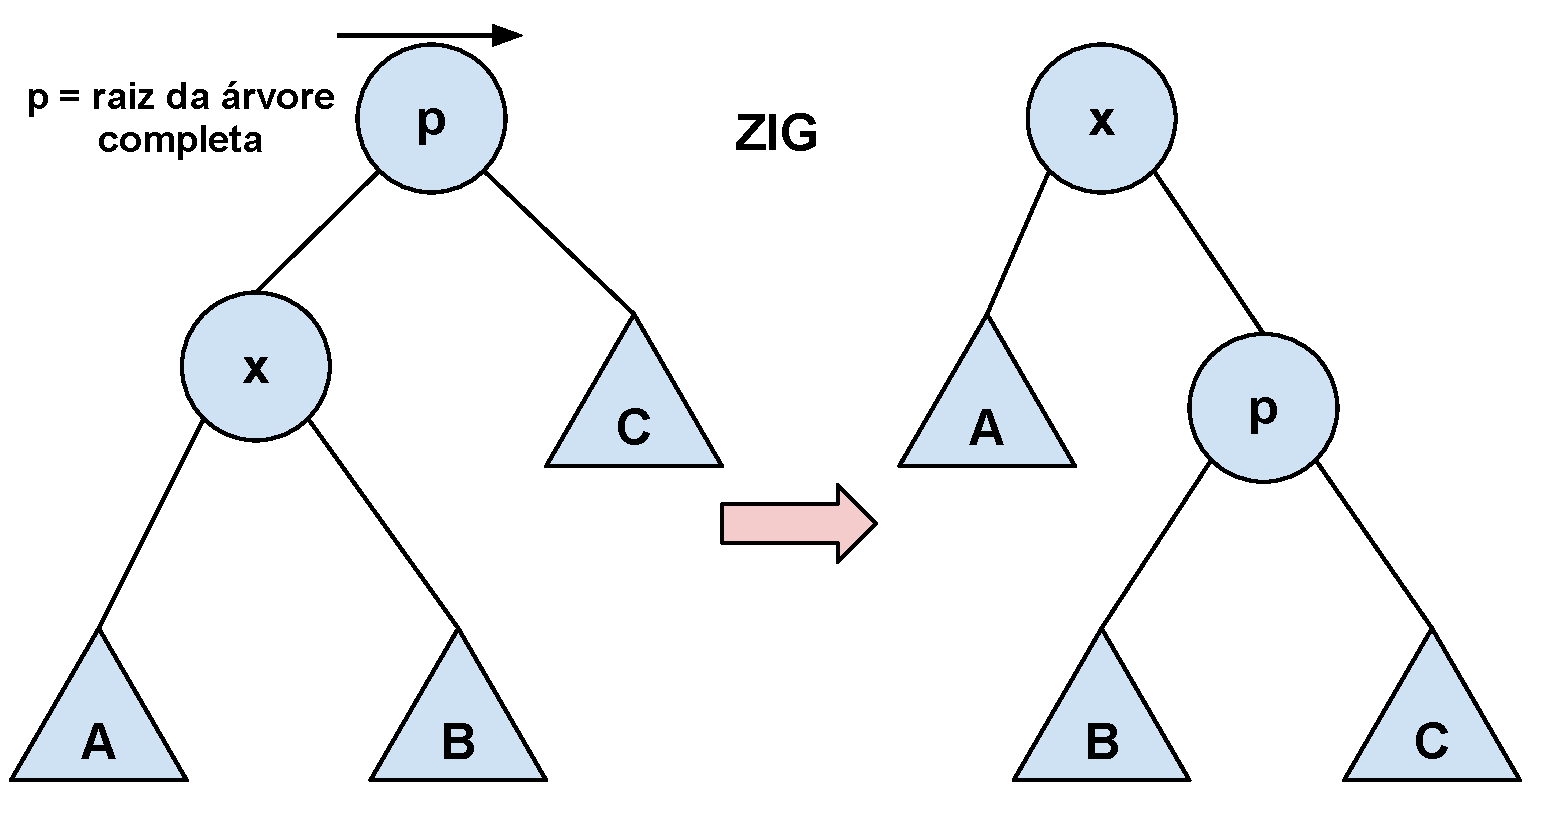
\includegraphics[keepaspectratio=true,width=4.5in]{figs/fig_arvores/Zig}
    \centering
    \end{figure}
}

%---------------------------------------------------------
\frame{
    \frametitle{Caso 2: ZIG-ZIG}
    
    \begin{figure}[tbp]
    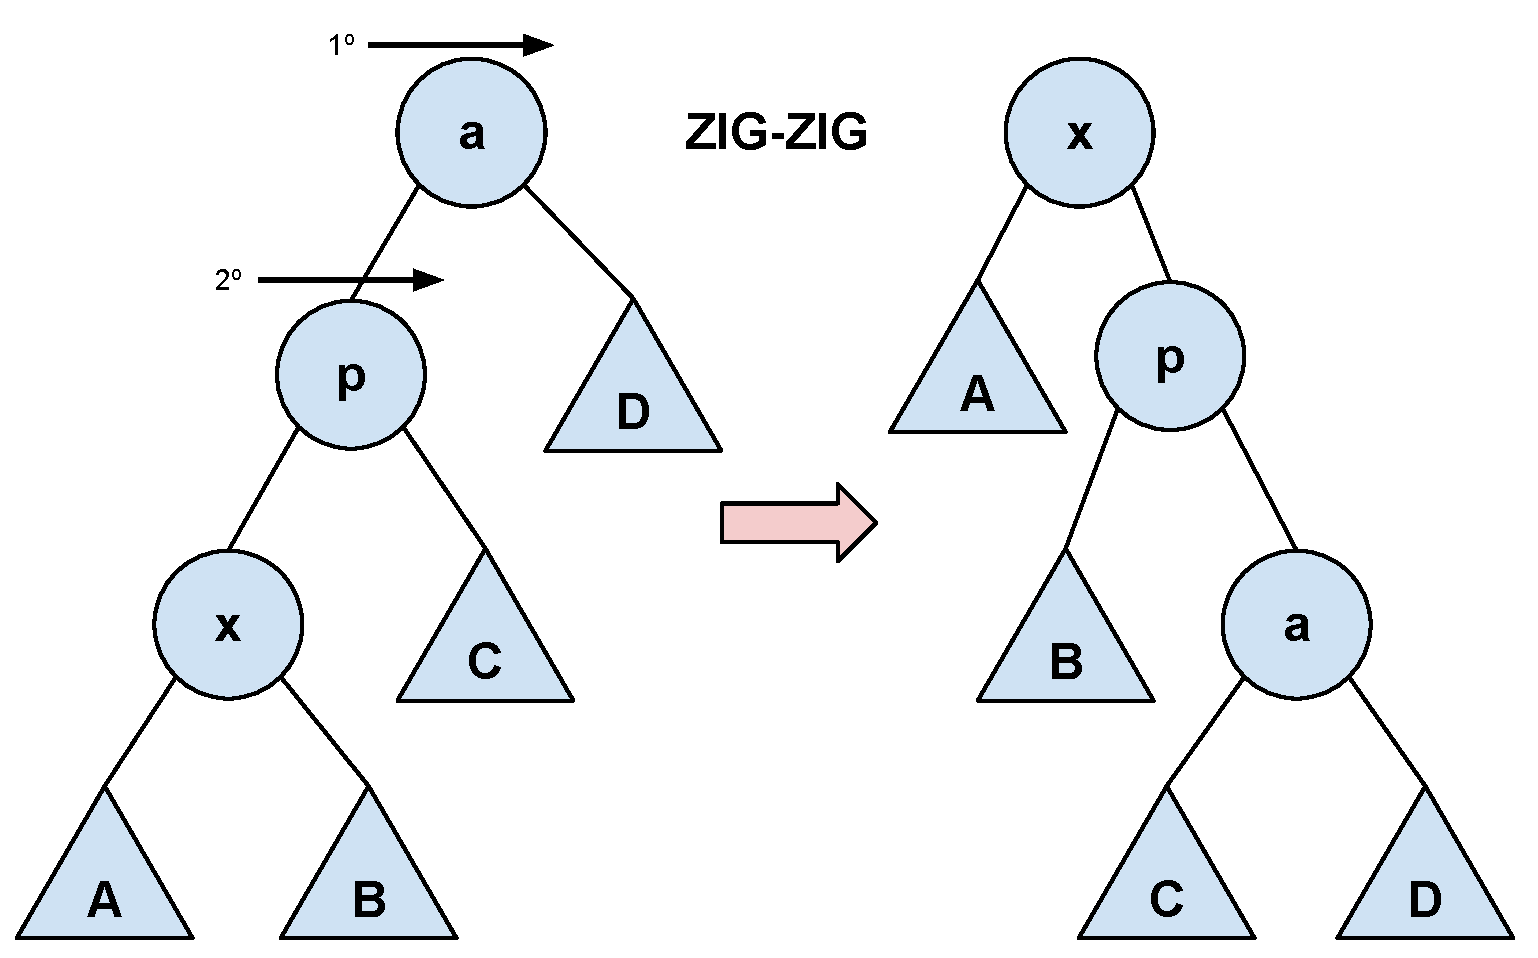
\includegraphics[keepaspectratio=true,width=4in]{figs/fig_arvores/Zig-Zig}
    \centering
    \end{figure}
}

%---------------------------------------------------------
\frame{
    \frametitle{Caso 3: ZIG-ZAG}
    
    \begin{figure}[tbp]
    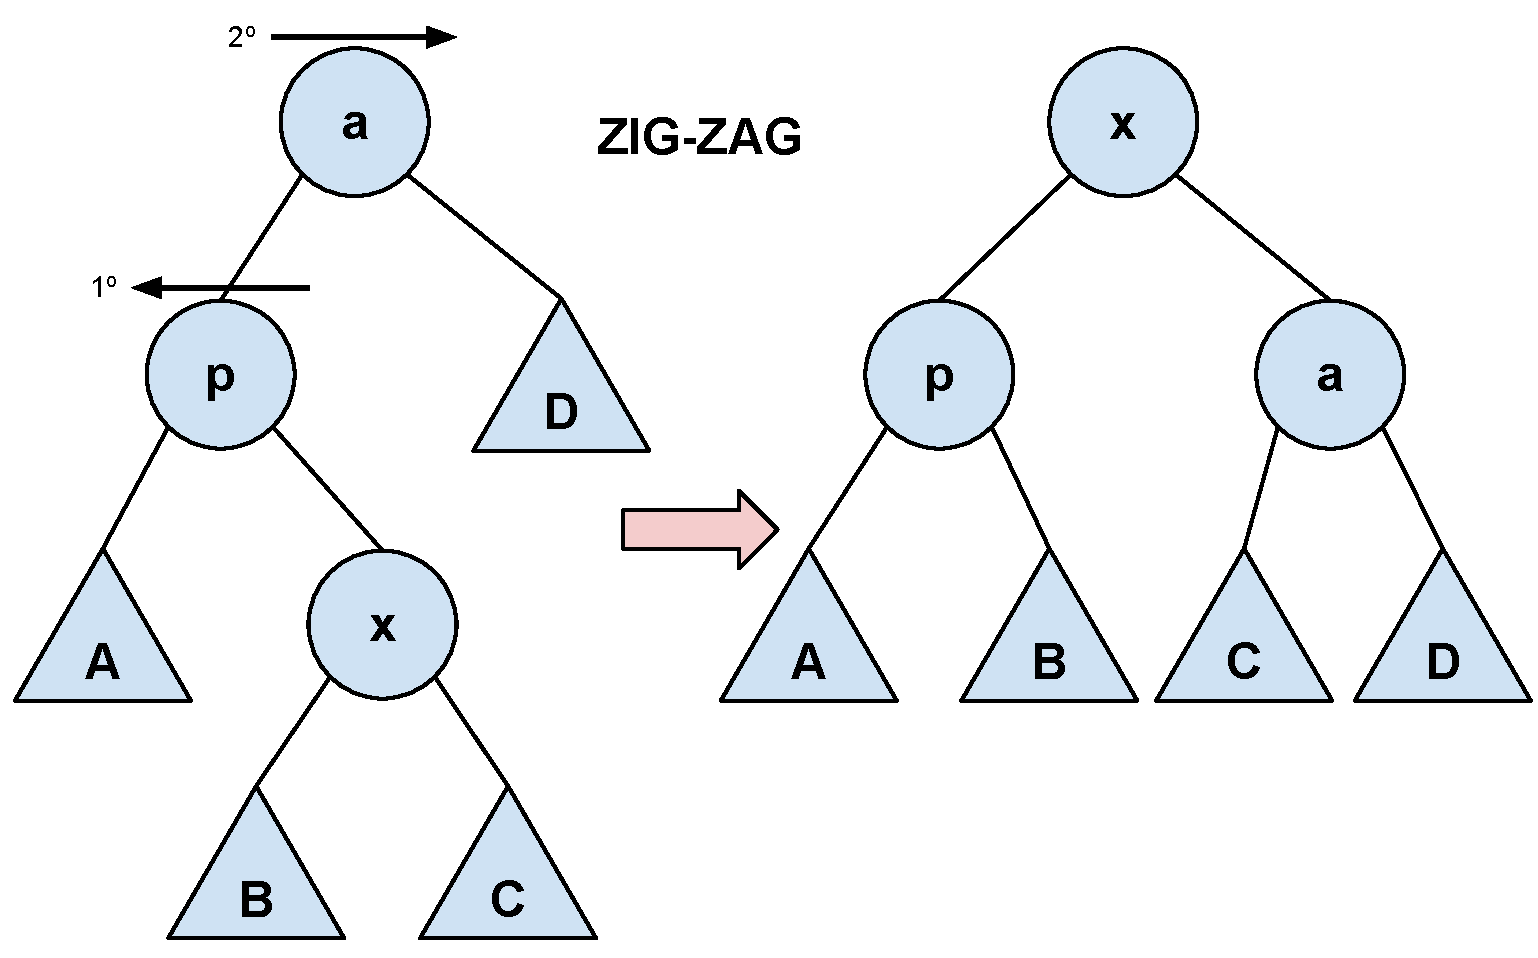
\includegraphics[keepaspectratio=true,width=4in]{figs/fig_arvores/Zig-Zag}
    \centering
    \end{figure}
}

%---------------------------------------------------------
\frame{
    \frametitle{Espalhamento Top-Down}
    
    \begin{itemize}
    \item Na estratégia Top-Down as chaves que estão no caminho da chave desejada
    para a raiz são rotacionadas e removidas para árvores auxiliares
    seguindo uma sequência de operações bem definidas
    \item Quando a chave desejada chega até a raiz, a árvore é remontada pelo
    retorno das chaves removidas
    \end{itemize}
}

%---------------------------------------------------------
\frame{
    \frametitle{Exemplo: Top-Down 1/6}
    
    \begin{figure}[tbp]
    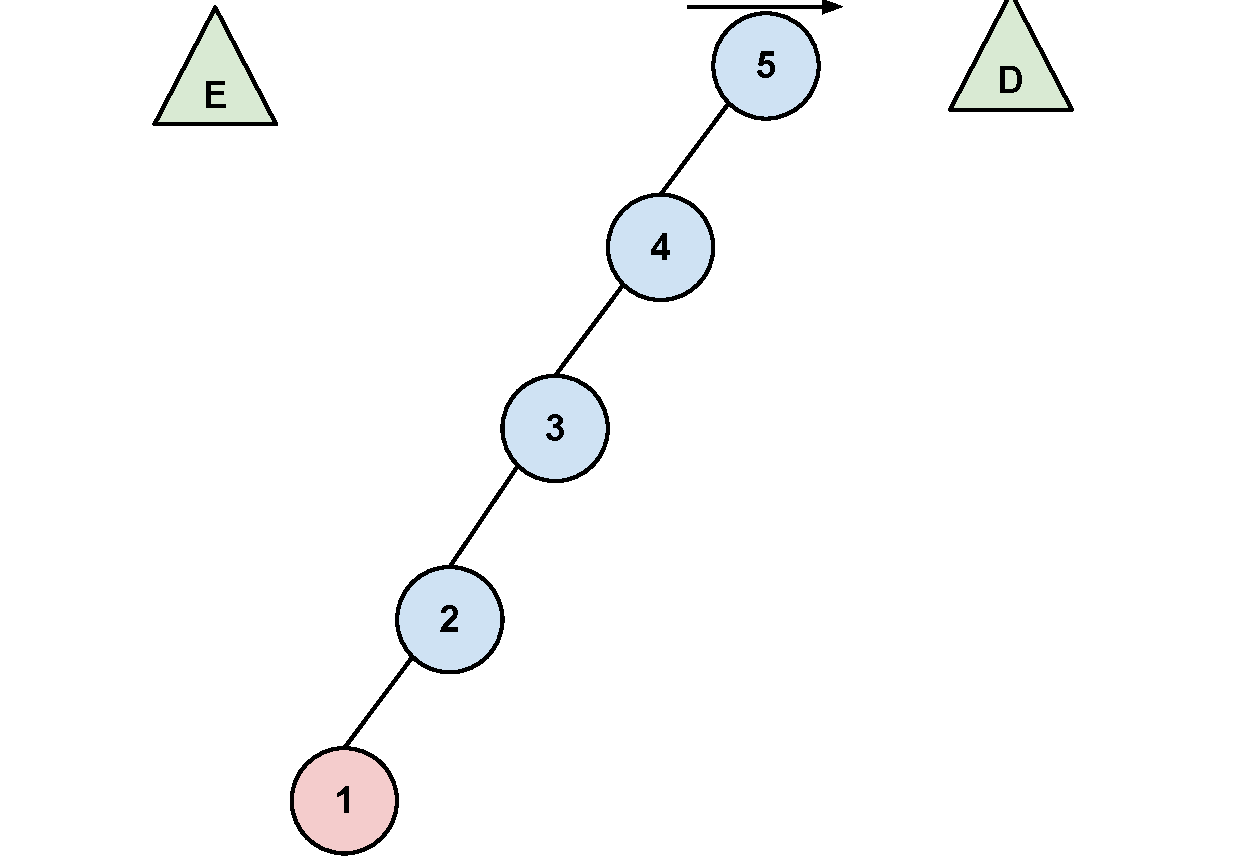
\includegraphics[keepaspectratio=true,width=3.5in]{figs/fig_arvores/Top-Down1}
    \centering
    \end{figure}
}

%---------------------------------------------------------
\frame{
    \frametitle{Exemplo: Top-Down 2/6}
    
    \begin{figure}[tbp]
    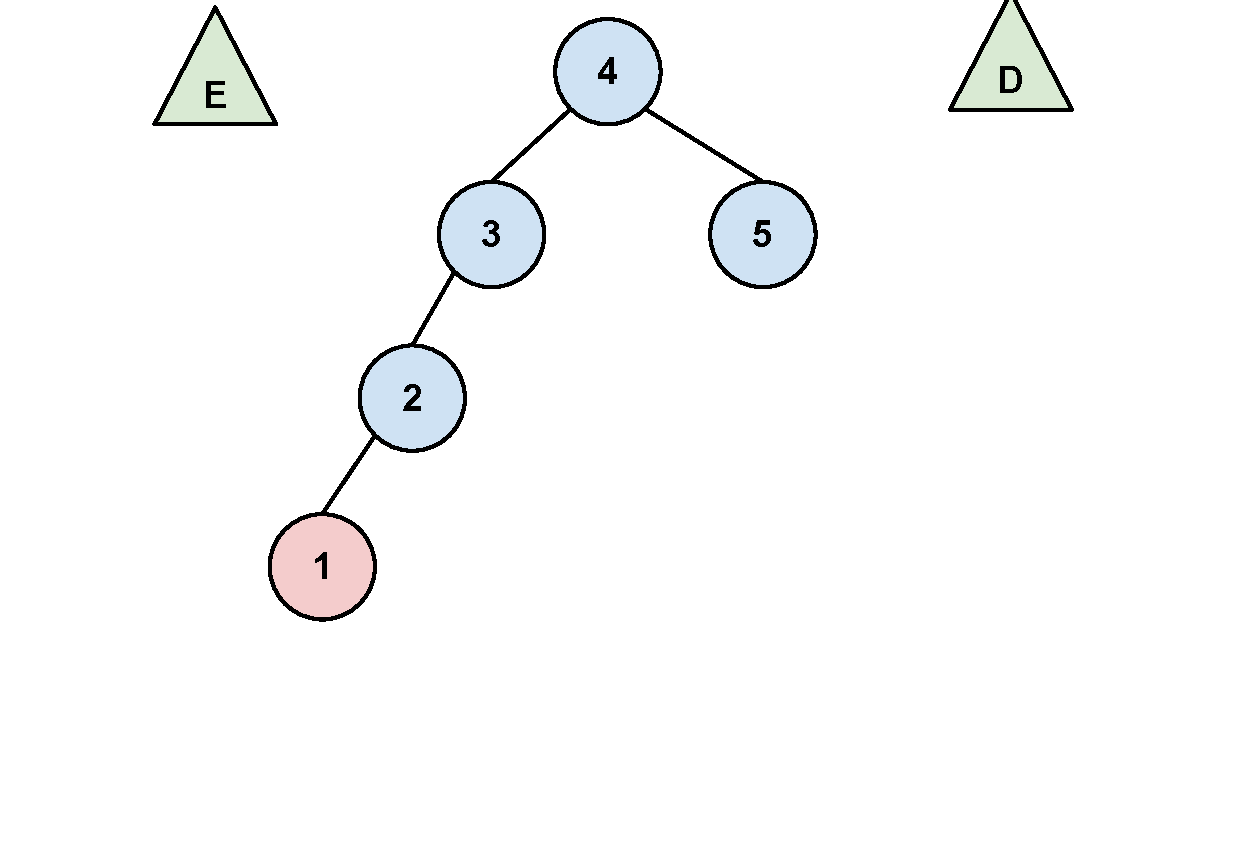
\includegraphics[keepaspectratio=true,width=3.5in]{figs/fig_arvores/Top-Down2}
    \centering
    \end{figure}
}

%---------------------------------------------------------
\frame{
    \frametitle{Exemplo: Top-Down 3/6}
    
    \begin{figure}[tbp]
    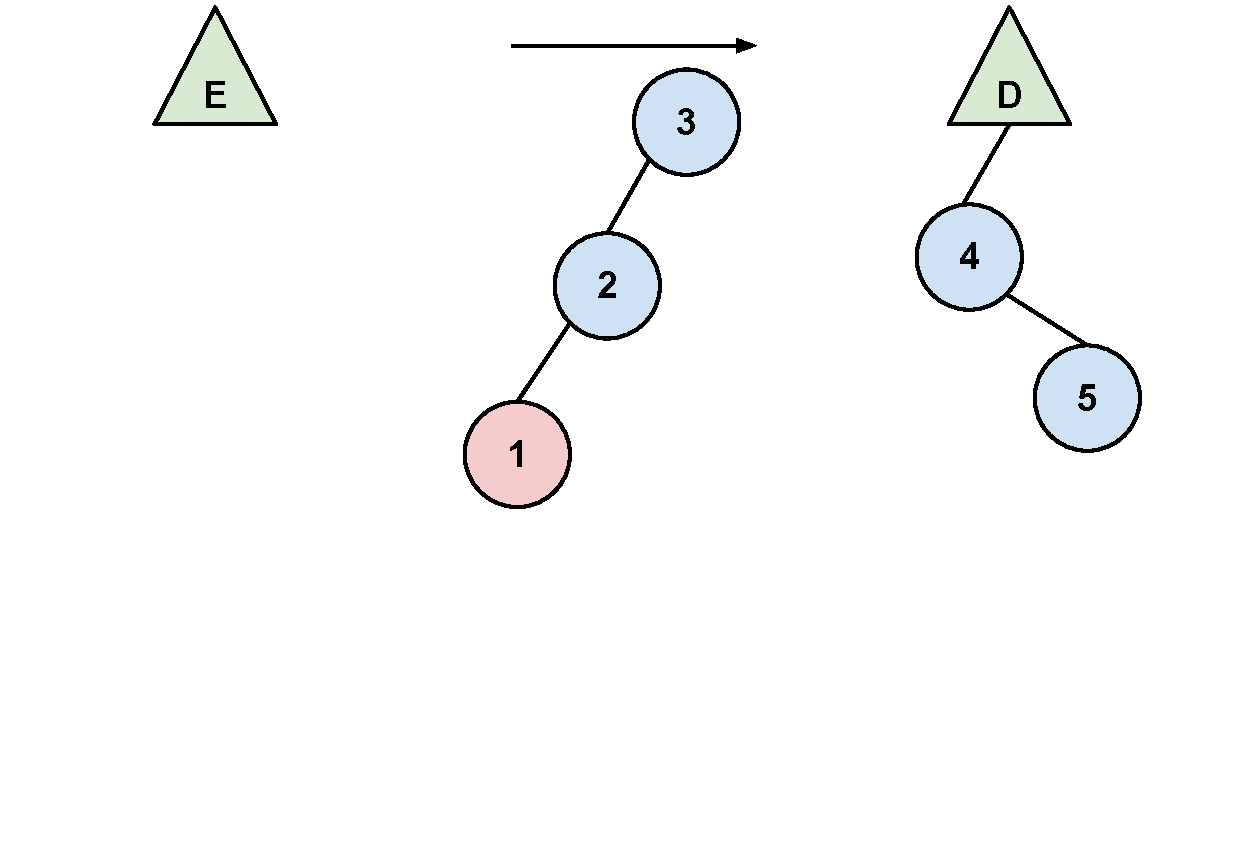
\includegraphics[keepaspectratio=true,width=3.5in]{figs/fig_arvores/Top-Down3}
    \centering
    \end{figure}
}

%---------------------------------------------------------
\frame{
    \frametitle{Exemplo: Top-Down 4/6}
    
    \begin{figure}[tbp]
    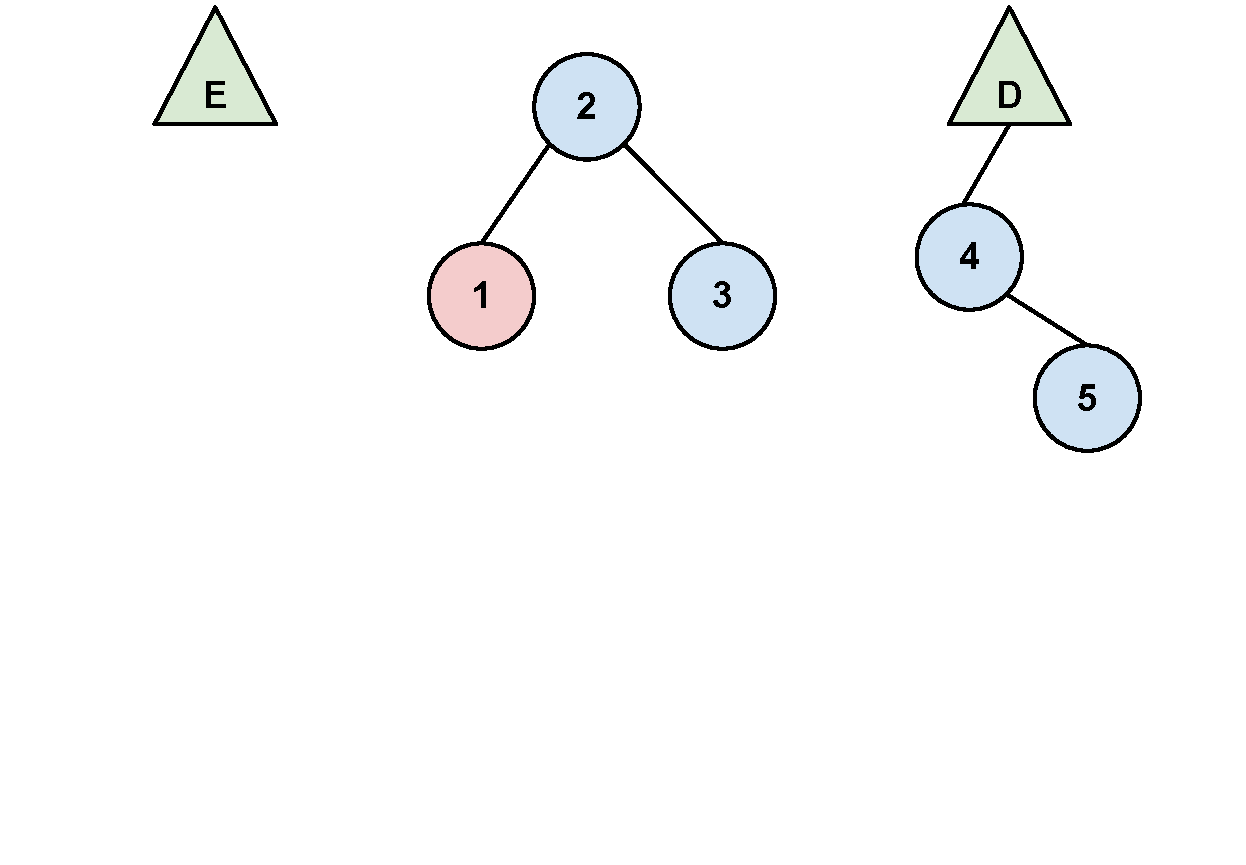
\includegraphics[keepaspectratio=true,width=3.5in]{figs/fig_arvores/Top-Down4}
    \centering
    \end{figure}
}

%---------------------------------------------------------
\frame{
    \frametitle{Exemplo: Top-Down 5/6}
    
    \begin{figure}[tbp]
    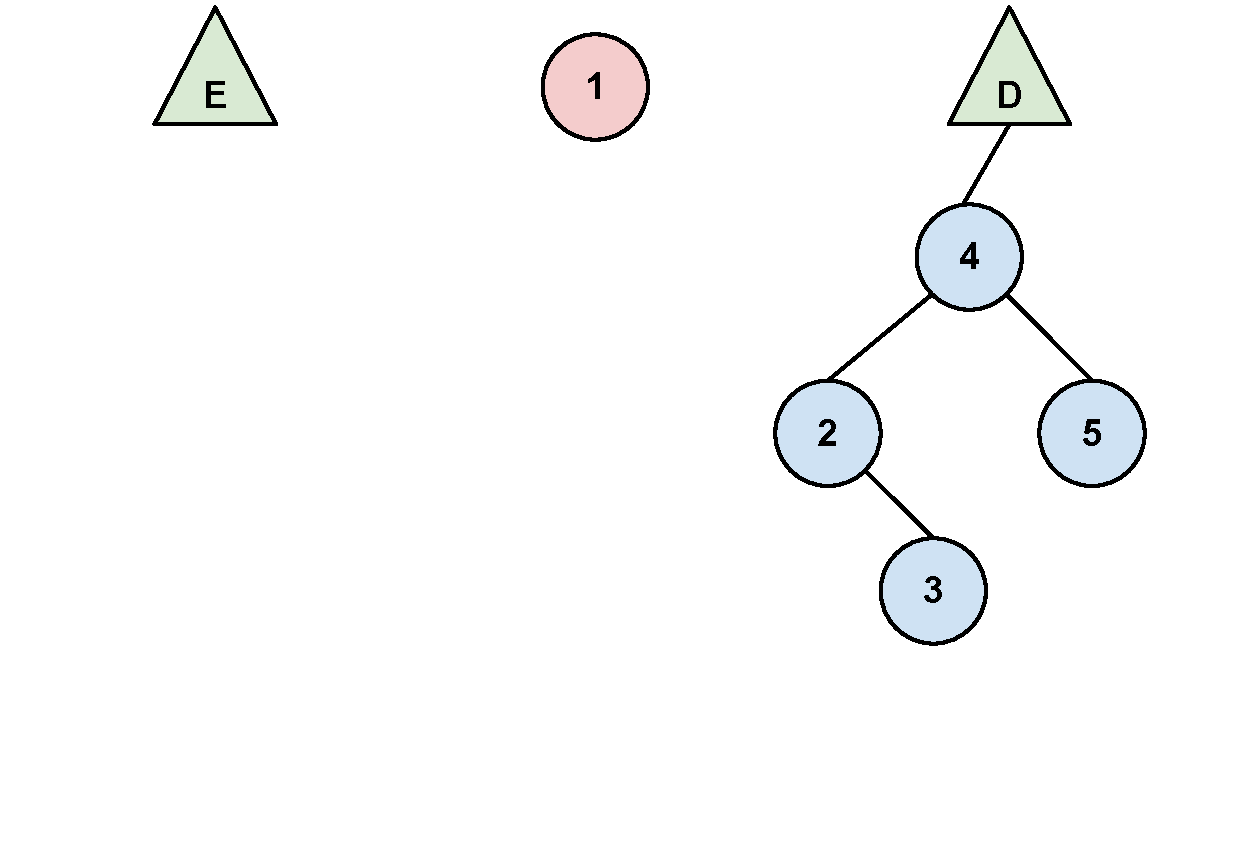
\includegraphics[keepaspectratio=true,width=3.5in]{figs/fig_arvores/Top-Down5}
    \centering
    \end{figure}
}

%---------------------------------------------------------
\frame{
    \frametitle{Exemplo: Top-Down 6/6}
    
    \begin{figure}[tbp]
    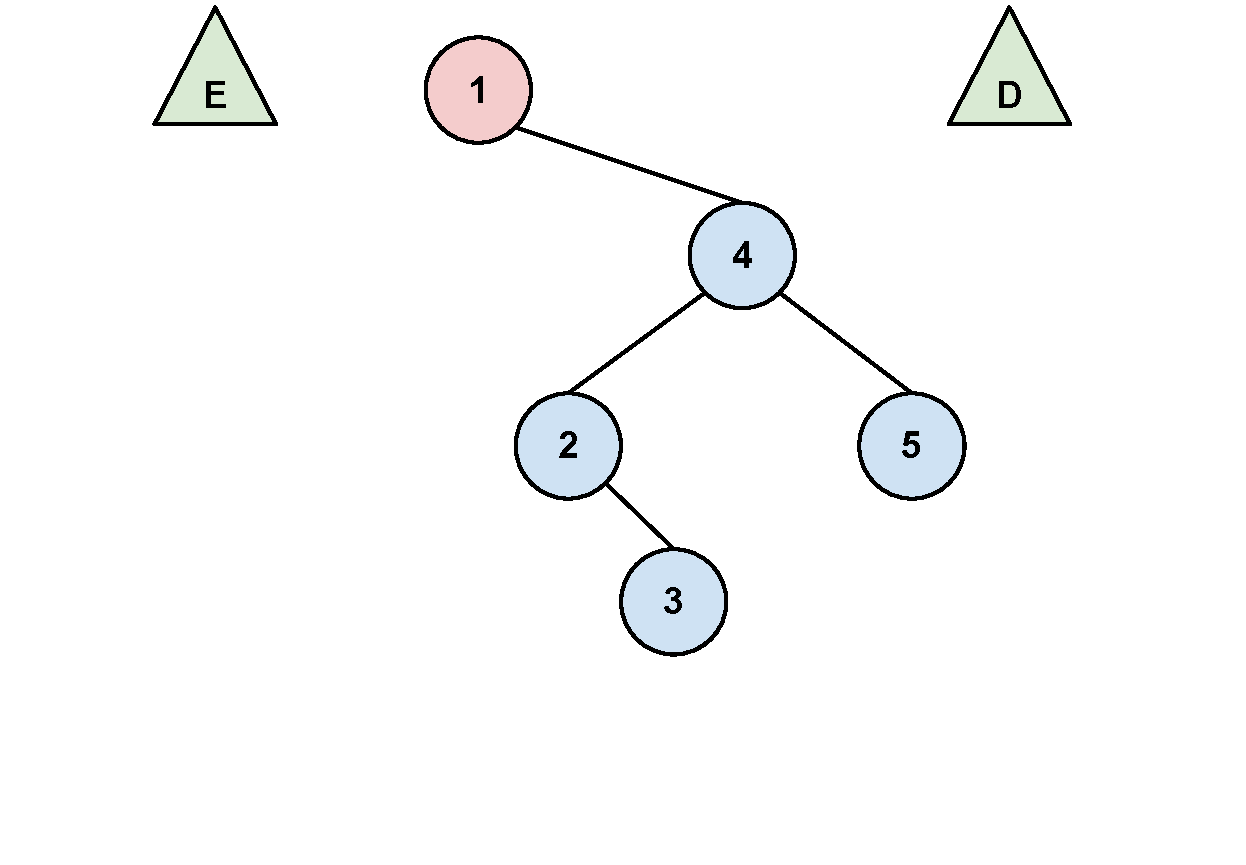
\includegraphics[keepaspectratio=true,width=3.5in]{figs/fig_arvores/Top-Down6}
    \centering
    \end{figure}
}




%---------------------------------------------------------
\begin{comment}
\section{Árvore B}

\bibliographystyle{unsrt}
\renewcommand\refname{Referências}

\frame{
    \frametitle{Referências}
    \bibliography{pres}
}

\end{comment}

%---------------------------------------------------------
